\documentclass{report}
\usepackage{imakeidx}
\usepackage[greek, english]{babel}
%\usepackage[T1]{fontenc}
\usepackage[utf8x]{inputenc}
\usepackage{amsthm}
%\usepackage{mbboard/texinputs/mbboard}
\usepackage{amssymb}
\usepackage{amsmath}
\usepackage{thmtools}
\usepackage{mathtools}
\usepackage{etoolbox}
\usepackage{scalerel}
\usepackage{siunitx}
\usepackage{tikz}
\usepackage{ulem}
\usepackage{contour}
\usepackage{xcolor}
\usepackage{bbold}
\usepackage{url}
\usepackage{slashed}
\usepackage{simpler-wick}
\usepackage{tikz-feynman}
\usepackage{../tikz-uml}
\usepackage{cancel}
\usepackage{graphicx}
\usepackage{wrapfig}
\usepackage{csquotes}
%\usepackage{commath}
\usepackage{subcaption}
\usepackage{pgfplots}
\usepackage{tensor}
\usepackage{verbatim}
\usepackage{esint}
\usepackage[shortlabels]{enumitem}
\usepackage[skins, breakable]{tcolorbox}
%\usepackage{bbm}
\usepackage{bm}
%\usepackage{autonum}
\usepackage{diagbox}


\usepackage{listings}
\usepackage[]{algorithm2e}

\usepackage[margin=1.4in]{geometry}
\usepackage[hidelinks, hypertexnames=false]{hyperref}
\usepackage[user, xr]{zref}

\makeindex[name=definition,title={Index of definitions}]

\tcbset{breakable}

\usetikzlibrary{cd, fit, patterns, snakes, decorations.markings, trees}
\usepgfmodule{nonlineartransformations}


% --- Theorems and such ---
\newtheorem{theorem}{Theorem}[part]
\newtheorem{corollary}{Corollary}[theorem]
\newtheorem{lemma}[theorem]{Lemma}
\newtheorem*{lemma*}{Lemma}
\newtheorem{proposition}[theorem]{Proposition}
%\newtheorem*{remark}{Remark} %Does not work (some package conflicts with amsthm)
% --- New commands ---
\newcommand{\R}{\mathbb{R}}
\newcommand{\N}{\mathbb{N}}
\newcommand{\Z}{\mathbb{Z}}
\newcommand{\Q}{\mathbb{Q}}
\newcommand{\C}{\mathbb{C}}
%\newcommand{\H}{\mathbb{H}}
\newcommand{\F}{\mathbb{F}}

\DeclarePairedDelimiter\ceil{\lceil}{\rceil}
\DeclarePairedDelimiter\floor{\lfloor}{\rfloor}

\DeclareMathOperator{\fractional}{frac}
\DeclareMathOperator{\integer}{int}

\newcommand{\transp}{\mathrm{T}}

% --- Inner products / brackets ---
\newcommand{\inner}[1]{\left\langle #1 \right\rangle}
\newcommand{\ket}[1]{\left| #1 \right\rangle}
\newcommand{\bra}[1]{\left\langle #1 \right|}
\newcommand{\braket}[3][\null]{%    %TOreDO!
  \ifx#1\null
       \langle#2|#3\rangle%
    \else%
       \langle#2|#1|#3\rangle%
    \fi}
\newcommand{\sbraket}[3][\null]{%    %TOreDO!
  \ifx#1\null
       \left\langle#2\vphantom{#3}\right.\left|#3\vphantom{#2}\right\rangle%
    \else%
         \left\langle#2\vphantom{#1}\vphantom{#3}\right.\left|#1\vphantom{#2}\vphantom{#3}\right|\left.#3\vphantom{#1}\vphantom{#2}\right\rangle%
    \fi}
\newcommand{\ketbra}[2]{|#1\rangle\langle#2|}
\newcommand{\sketbra}[2]{\left|#1\vphantom{#2}\right\rangle\left\langle#2\vphantom{#1}\right|}

\newcommand{\grade}[1]{\left\langle #1 \right\rangle}
% --- Set builder notation ---
\newcommand{\setbuilder}[2]{ \left\{\left. #1 \;\right|\; #2 \right\} }
% --- Script r ---
\def\rcurs{{\mbox{$\resizebox{.09in}{.08in}{
\includegraphics[trim= 1em 0 14em 0,clip]{ScriptR}}$}}}
\def\brcurs{{\mbox{$\resizebox{.09in}{.08in}{
\includegraphics[trim= 1em 0 14em 0,clip]{BoldR}}$}}}
\def\hrcurs{{\mbox{$\hat \brcurs$}}}
% --- Vector style ---
\let\arrowvec\vec
\renewcommand{\vec}[1]{\bm{\mathrm{#1}}}
%\let\ihat\hat
%\let\operator\hat
\newcommand{\vhat}[1]{\vec{\hat{#1}}}
% --- Complex vectors ---
\newcommand{\vbar}[1]{\vec{\bar{#1}}}
% --- Norm ---
\makeatletter
\DeclareDocumentCommand\braces{}{{\ifnum\z@=`}\fi\@braces}
\DeclareDocumentCommand\@braces{ s t\big t\Big t\bigg t\Bigg m m m }
{ % General braces with automatic and manual sizing
	\IfBooleanTF{#1}
	{\left#6\smash{#8}\right#7\vphantom{#8}}
	{
		\IfBooleanTF{#2}{\bigl#6{#8}\bigr#7}{
			\IfBooleanTF{#3}{\Bigl#6{#8}\Bigr#7}{
				\IfBooleanTF{#4}{\biggl#6{#8}\biggr#7}{
					\IfBooleanTF{#5}{\Biggl#6{#8}\Biggr#7}{\left#6{#8}\right#7}
				}
			}
		}
	}
	\ifnum\z@=`{\fi}
}
%\DeclareDocumentCommand\norm{ l m }{\braces#1{\lVert}{\rVert}{#2}} % Norm
\makeatother

\newcommand\swapifbranches[3]{#1{#3}{#2}}
\makeatletter
\MHInternalSyntaxOn
\patchcmd{\DeclarePairedDelimiter}{\@ifstar}{\swapifbranches\@ifstar}{}{}
\MHInternalSyntaxOff
\makeatother

\DeclarePairedDelimiter{\norm}{\lVert}{\rVert}
% --- Lines in (block) matrices ---
% --- Defining quantities ---
\newcommand{\defeq}{\coloneqq}
\newcommand{\eqdef}{\eqqcolon}
\newcommand{\defequiv}{\quad\Leftrightarrow_{\text{def}}\quad}
% --- Maths operators ---
\DeclareMathOperator{\Set}{Set}
\DeclareMathOperator{\acc}{acc}
\newcommand\powerset{\mathop{\mathcal{P}}}
\newcommand{\symdiff}{\mathbin{\Delta}}

\DeclareMathOperator{\graph}{graph}
\DeclareMathOperator{\len}{len}
\DeclareMathOperator{\seg}{seg}
\newcommand\seq[1]{\langle #1 \rangle}

\newcommand\cat[1]{\mathsf{#1}}
\DeclareMathOperator{\ob}{ob}
\DeclareMathOperator{\mor}{mor}

\DeclareMathOperator\id{id}
\DeclareMathOperator\dom{dom}
\DeclareMathOperator\codom{codom}
\DeclareMathOperator\co{co}
\DeclareMathOperator\im{im}
\DeclareMathOperator\evalMap{ev}

\DeclareMathOperator\Hom{Hom}

\DeclareMathOperator{\lcm}{lcm}
%\DeclareMathOperator{\gcd}{gcd}

\newcommand\ideals{\mathop{\mathcal{I}}}
\newcommand\filters{\mathop{\mathcal{F}}}

\newcommand\joinIr{\mathop{\mathcal{J}}}
\newcommand\meetIr{\mathop{\mathcal{M}}}

\newcommand\neighbourhoods{\mathop{\mathcal{N}}}
\DeclareMathOperator{\closure}{Cl}

\DeclareMathOperator{\st}{st}

\DeclareMathOperator{\group}{gp}

\let\Im\relax
\DeclareMathOperator\Im{\mathfrak{I}m}
\let\Re\relax
\DeclareMathOperator\Re{\mathfrak{R}e}

%\renewcommand{\Re}{\operatorname{Re}}
%\renewcommand{\Im}{\operatorname{Im}}

\DeclareMathOperator{\SF}{SF}

\DeclareMathOperator{\GL}{GL}
\DeclareMathOperator{\SL}{SL}
\DeclareMathOperator{\Ogroup}{O}
\DeclareMathOperator{\SO}{SO}
\DeclareMathOperator{\SU}{SU}
\DeclareMathOperator{\U}{U}

\DeclareMathOperator{\Iso}{Iso}

\DeclareMathOperator{\Pin}{Pin}
\DeclareMathOperator{\Spin}{Spin}

\DeclareMathOperator{\glAlg}{gl}
\DeclareMathOperator{\slAlg}{sl}
\DeclareMathOperator{\uAlg}{u}
\DeclareMathOperator{\suAlg}{su}
\DeclareMathOperator{\oAlg}{o}
\DeclareMathOperator{\soAlg}{so}

\DeclareMathOperator{\diag}{diag}
\DeclareMathOperator{\Ad}{Ad}
\DeclareMathOperator{\ad}{ad}
\DeclareMathOperator{\sgn}{sgn}
\DeclareMathOperator\atanh{arctanh}
\DeclareMathOperator\sech{sech}
\DeclareMathOperator\csch{csch}

\DeclareMathOperator\Span{span}
\newcommand\Lin{\mathop{\mathcal{L}}}
\DeclareMathOperator\codim{codim}
\DeclareMathOperator\coker{coker}

\DeclareMathOperator\NumRange{W}
\DeclareMathOperator\nr{nr}

\DeclareMathOperator\Row{row}
\DeclareMathOperator\Col{col}
\DeclareMathOperator\Null{null}
\DeclareMathOperator\Rank{rank}
\DeclareMathOperator\KruskalRank{K}

\newcommand\Expval[1]{\mathbb{E}\left[#1\right]}
\newcommand\expval[1]{\left\langle #1 \right\rangle}
\DeclareMathOperator\Var{Var}

\DeclareMathOperator\vectorisation{vec}
\DeclareMathOperator\Tr{Tr}
\DeclareMathOperator\adj{adj}
\DeclareMathOperator\End{End}
\DeclareMathOperator\Aut{Aut}
\newcommand\Bounded{\mathop{\mathcal{B}}}
\newcommand\Compact{\mathop{\mathcal{K}}}
\newcommand\Fred{\mathop{\mathcal{F}}}

\newcommand\cont{\mathop{\mathcal{C}}}
\newcommand\testFuncs{\mathop{\mathcal{D}}}
\newcommand\dists{\mathop{\mathcal{D}^\prime}}

\DeclareMathOperator\Cl{Cl}
\DeclareMathOperator\cCl{\mathbb{C}l}

\DeclareMathOperator\Ind{Ind}
\DeclareMathOperator\Index{idx}

\NewDocumentCommand{\grad}{}{%
  \mathop{}\!% \mathop for good spacing before \nabla
  \nabla}
\NewDocumentCommand{\curl}{}{%
  \mathop{}\!% \mathop for good spacing before \nabla
  \nabla\times}
\DeclareMathOperator\vnabla{\vec{\nabla}}

\DeclareMathOperator\Res{Res}

\newcommand\Normals{\mathop{\mathcal{N}}\nolimits}
\newcommand\SelfAdjoints{\mathop{\mathcal{SA}}\nolimits}
\newcommand\Projections{\mathop{\mathcal{P}}\nolimits}
\newcommand\Unitaries{\mathop{\mathcal{U}}\nolimits}

% --- Algebraic dual / topological dual / commutant ---
\DeclareMathSymbol{\mlq}{\mathord}{operators}{``}
\DeclareMathSymbol{\mrq}{\mathord}{operators}{`'}

\newcommand\adual[1]{{#1}^*}
\newcommand\abidual[1]{{#1}^{**}}
\newcommand\tdual[1]{{#1}^\prime}
\newcommand\tbidual[1]{{#1}^{\prime\prime}}
\newcommand\comm[1]{{#1}\raisebox{-0.15em}{$\scaleobj{1.3}{\mrq}$}}
% --- Define custom environments ---
\newtcolorbox{note}{enhanced,sharp corners=all,colback=white,colframe=black,toprule=-1pt,bottomrule=-1pt,leftrule=1pt,rightrule=-1pt, overlay unbroken={
\draw[black,line width=1pt] (frame.north west) -- ++(.2,0);
\draw[black,line width=1pt] (frame.south west) -- ++(.2,0);
}, overlay first={
\draw[black,line width=1pt] (frame.north west) -- ++(.2,0);
}, overlay last={
\draw[black,line width=1pt] (frame.south west) -- ++(.2,0);
}, left=2mm, top=2mm, bottom=2mm}

%\newtcolorbox{practical}{enhanced,sharp corners=all,colback=white,colframe=black,toprule=0pt,bottomrule=0pt,leftrule=1pt,rightrule=0pt, overlay unbroken={
%\draw[black,line width=1pt] (frame.north west) -- ++(.2,0);
%\draw[black,line width=1pt] (frame.south west) -- ++(.2,0);
%}, overlay first={
%\draw[black,line width=1pt] (frame.north west) -- ++(.2,0);
%}, overlay last={
%\draw[black,line width=1pt] (frame.south west) -- ++(.2,0);
%}, left=2mm, top=2mm, bottom=2mm}

\newtcolorbox{example}{enhanced,sharp corners=all,colback=white,colframe=black,toprule=-1pt,bottomrule=-1pt,leftrule=1pt,rightrule=-1pt, overlay unbroken={
\draw[black,line width=1pt] (frame.north west) -- ++(.2,0);
\draw[black,line width=1pt] (frame.south west) -- ++(.2,0);
}, overlay first={
\draw[black,line width=1pt] (frame.north west) -- ++(.2,0);
}, overlay last={
\draw[black,line width=1pt] (frame.south west) -- ++(.2,0);
}, title={\underline{Example}}, attach boxed title to top,
boxed title style={empty,size=minimal,toprule=2pt,top=4pt},
coltitle=black, left=2mm, top=2mm, bottom=2mm}

\newtcolorbox{params}{enhanced,sharp corners=all,colback=white,colframe=black,toprule=-1pt,bottomrule=-1pt,leftrule=1pt,rightrule=-1pt, overlay unbroken={
\draw[black,line width=1pt] (frame.north west) -- ++(.2,0);
\draw[black,line width=1pt] (frame.south west) -- ++(.2,0);
}, overlay first={
\draw[black,line width=1pt] (frame.north west) -- ++(.2,0);
}, overlay last={
\draw[black,line width=1pt] (frame.south west) -- ++(.2,0);
}, left=2mm, top=2mm, bottom=2mm}

\newtcolorbox{definition}{enhanced,sharp corners=all,colback=white,colframe=red,toprule=-1pt,bottomrule=-1pt,leftrule=1pt,rightrule=-1pt, overlay unbroken={
\draw[red,line width=1pt] (frame.north west) -- ++(.2,0);
\draw[red,line width=1pt] (frame.south west) -- ++(.2,0);
}, overlay first={
\draw[red,line width=1pt] (frame.north west) -- ++(.2,0);
}, overlay last={
\draw[red,line width=1pt] (frame.south west) -- ++(.2,0);
}, %title={DEF}, attach boxed title to top, boxed title style={empty,size=minimal,toprule=2pt,top=4pt}, coltitle=red, left=2mm, top=2mm, bottom=2mm
}

\newtcolorbox{eigenschap}{enhanced,sharp corners=all,colback=white,colframe=green,toprule=0pt,bottomrule=0pt,leftrule=1pt,rightrule=0pt, overlay unbroken={
\draw[green,line width=1pt] (frame.north west) -- ++(.2,0);
\draw[green,line width=1pt] (frame.south west) -- ++(.2,0);
}, overlay first={
\draw[green,line width=1pt] (frame.north west) -- ++(.2,0);
}, overlay last={
\draw[green,line width=1pt] (frame.south west) -- ++(.2,0);
}, left=2mm, top=2mm, bottom=2mm}
% --- Define underlines ---
\renewcommand{\ULdepth}{1.8pt}
\contourlength{0.9pt}
\renewcommand{\ULthickness}{.7pt}
\newcommand{\udef}[1]{%
\textcolor{red}{\uline{\phantom{#1}}}%
  \llap{\contour{white}{#1}}%
\index[definition]{#1}%
}
\newcommand{\ueig}[1]{%
\textcolor{green}{\uline{\phantom{#1}}}%
  \llap{\contour{white}{#1}}%
}
\newcommand{\undline}[1]{%
\uline{\phantom{#1}}%
  \llap{\contour{white}{#1}}%
}
% --- Important remark ---
\newcommand{\remark}[1]{\begin{center}\textbf{#1}\end{center}}
% --- Extra symbols ---
\newcommand*{\twoheadrightarrowtail}{\mathrel{\rightarrowtail\kern-1.9ex\twoheadrightarrow}}

\DeclareFontFamily{U}{mathb}{\hyphenchar\font45}
\DeclareFontShape{U}{mathb}{m}{n}{
      <5> <6> <7> <8> <9> <10> gen * mathb
      <10.95> mathb10 <12> <14.4> <17.28> <20.74> <24.88> mathb12
      }{}
\DeclareSymbolFont{mathb}{U}{mathb}{m}{n}
\DeclareFontSubstitution{U}{mathb}{m}{n}
\DeclareMathSymbol{\sqsubsetneq}    {3}{mathb}{"88}


\DeclareFontFamily{OT1}{mbb}{\hyphenchar\font45}
%
\DeclareFontShape{OT1}{mbb}{m}{n}{
      <5> <6> <7> <8> <9> <10> gen * mbb
      <10.95> mbb10 <12> <14.4> mbb12 <17.28> <20.74> <24.88> mbb17
      }{}
\DeclareSymbolFont{mbb}{OT1}{mbb}{m}{n}
%
\DeclareFontShape{OT1}{mbb}{bx}{n}{
      <5> <6> <7> <8> <9> <10> gen * mbb
      <10.95> mbb10 <12> <14.4> mbb12 <17.28> <20.74> <24.88> mbb17
      }{}
\DeclareSymbolFont{mbb}{OT1}{mbb}{bx}{n}


\DeclareMathSymbol{\bbomega}{0}{mbb}{"B8}
% --- Defines pictures and graphics ---
\makeatletter
\def\circletransformation{%
\pgfmathsetmacro{\myX}{\pgf@x*sin(\pgf@y)*.6}
\pgfmathsetmacro{\myY}{\pgf@x*cos(\pgf@y)*.6}
\setlength{\pgf@x}{\myX pt}
\setlength{\pgf@y}{\myY pt}
}
\makeatother

\tikzset{
  apple/.pic={
    \draw (0,1) .. controls (-.6,1.8) and (-1.3,.8) .. (-1.1,0) .. controls (-.9,-.8) and (-.3,-1.5) .. (0,-1) .. controls (.3,-1.5) and (.9,-.8) .. (1.1,0) .. controls (1.3,.8) and (.6,1.8) .. (0,1) -- (0,1.6);
  }
}
% --- More settings ---
\newlength\tindent
\setlength{\tindent}{\parindent}
\setlength{\parindent}{0pt}
\renewcommand{\indent}{\hspace*{\tindent}}

% Start at chapter zero:
\setcounter{chapter}{-1}

% Include \paragraph in ToC:
\setcounter{tocdepth}{5}
% Number \subsubsection:
\setcounter{secnumdepth}{3}

\graphicspath{ {./images/} }

% =========================== Commath clone ========================
% Differential (upface d)
\DeclareMathOperator{\diff}{d \!}
% Derivative (upface D)
\DeclareMathOperator{\Diff}{D \!}

% Command for partial derivatives. The first argument denotes the function and the second argument denotes the variable with respect to which the derivative is taken. The optional argument denotes the order of differentiation. The style (text style/display style) is determined automatically
\providecommand{\pd}[3][]{\ensuremath{
\frac{\partial{^{#1}}#2}{\partial{{#3}^{#1}}}
}}

% \tpd[2]{f}{k} denotes the second partial derivative of f with respect to k
% The first letter t means "text style"
\providecommand{\tpd}[3][]{\ensuremath{\mathinner{
\tfrac{\partial{^{#1}}#2}{\partial{{#3}^{#1}}}
}}}
% \dpd[2]{f}{k} denotes the second partial derivative of f with respect to k
% The first letter d means "display style"
\providecommand{\dpd}[3][]{\ensuremath{\mathinner{
\dfrac{\partial{^{#1}}#2}{\partial{{#3}^{#1}}}
}}}

% mixed derivative - analogous to the partial derivative command
% \md{f}{5}{x}{2}{y}{3}
\providecommand{\md}[6]{\ensuremath{
\ifinner
\tfrac{\partial{^{#2}}#1}{\partial{{#3}^{#4}}\partial{{#5}^{#6}}}
\else
\dfrac{\partial{^{#2}}#1}{\partial{{#3}^{#4}}\partial{{#5}^{#6}}}
\fi
}}

% \tpd[2]{f}{k} denotes the second partial derivative of f with respect to k
% The first letter t means "text style"
\providecommand{\tmd}[6]{\ensuremath{\mathinner{
\tfrac{\partial{^{#2}}#1}{\partial{{#3}^{#4}}\partial{{#5}^{#6}}}
}}}
% \dpd[2]{f}{k} denotes the second partial derivative of f with respect to k
% The first letter d means "display style"
\providecommand{\dmd}[6]{\ensuremath{\mathinner{
\dfrac{\partial{^{#2}}#1}{\partial{{#3}^{#4}}\partial{{#5}^{#6}}}
}}}


% ordinary derivative - analogous to the partial derivative command
\providecommand{\od}[3][]{\ensuremath{
\ifinner
\tfrac{\diff{^{#1}}#2}{\diff{{#3}^{#1}}}
\else
\dfrac{\diff{^{#1}}#2}{\diff{{#3}^{#1}}}
\fi
}}

\providecommand{\tod}[3][]{\ensuremath{\mathinner{
\tfrac{\diff{^{#1}}#2}{\diff{{#3}^{#1}}}
}}}
\providecommand{\dod}[3][]{\ensuremath{\mathinner{
\dfrac{\diff{^{#1}}#2}{\diff{{#3}^{#1}}}
}}}

% functional derivative - analogous to the partial derivative command
\providecommand{\fd}[3][]{\ensuremath{
\ifinner
\tfrac{\delta{^{#1}}#2}{\delta{{#3}^{#1}}}
\else
\dfrac{\delta{^{#1}}#2}{\delta{{#3}^{#1}}}
\fi
}}

\providecommand{\tfd}[3][]{\ensuremath{\mathinner{
\tfrac{\delta{^{#1}}#2}{\delta{{#3}^{#1}}}
}}}
\providecommand{\dfd}[3][]{\ensuremath{\mathinner{
\dfrac{\delta{^{#1}}#2}{\delta{{#3}^{#1}}}
}}}

% --- Code style ---
\lstdefinestyle{program}{numbers=left}
\lstdefinestyle{snippet}{}
\usepackage{courier}
\definecolor{verylightgray}{gray}{0.95}
\lstset{basicstyle=\selectfont\ttfamily, backgroundcolor=\color{verylightgray}}
% --- Syntax environment ---
\newenvironment{syntax}{\begin{center}\ttfamily \small}{\end{center}}
\newcommand{\opt}[1]{\textbf{(}#1\textbf{)?}}
\newcommand{\optnb}[1]{#1\textbf{?}}
\newcommand{\mult}[1]{\textbf{(}#1\textbf{)*}}
\newcommand{\multnb}[1]{#1\textbf{*}}
\newcounter{index}
\newcommand\opts[1]{%
  \getargsC{#1}%
  \textbf{(} \argi%
  \setcounter{index}{1}
  \whiledo{\value{index} < \narg}{%
    \stepcounter{index}%
     \textbf{|} \csname arg\romannumeral\value{index}\endcsname \hspace{.8em}%
  }\textbf{)}%
}



% --- End setup ---

\zexternaldocument*[math-]{../Mathematics/TheBigIdeas_Mathematics}

\title{Some of the Big Ideas in Computer Science}
\author{Joseph Cunningham}
\date{}

\begin{document}
\maketitle
\tableofcontents

Clean architecture

Gang of four

TODO: unity of terminology!

\part{Background}
\setcounter{chapter}{0} % Reset chapter counter
\chapter{What is a computer?}
What is data? Also binary
Turing machine: undecidability, the halting problem, 
Lambda calculus
Abacus
Von Neumann / computer architecture (+infra)
Church-turing thesis (+ materialism?)
Minimal working computer

\chapter{Organization of computer systems}
A computer system can be divided roughly into four components:
\begin{enumerate}
\item The hardware;
\item The operating system;
\item The application programs;
\item The users.
\end{enumerate}

\section{Hardware}
\subsection{The CPU}
assembly / machine language

address of execution / program counter

\subsection{Storage}
Pointers

\subsubsection{Design parameters}
\begin{itemize}
\item Speed (read / write)
\item Size
\item Volatility
\item Ability to be written to (yes - RW / no / limited - WORM)
\end{itemize}

\subsubsection{Types of storage}
\paragraph{ROM}
Also EEPROM. Firmware.
\paragraph{Registers}
\paragraph{Cache}
\paragraph{Main memory (RAM)}
\paragraph{Secondary memory}
\paragraph{External (tertiary) storage}

\subsection{I/O devices and controllers}

\section{Computer-system architecture}
TODO: what is it? Configuration of pieces of hardware.
\subsection{System design}
\subsubsection{Computing environments}
\paragraph{Traditional computing}
\paragraph{Mobile computing} Includes GPS, accelerometers etc.
\paragraph{Distributed systems} Networks characterised based on distance between nodes:
\begin{itemize}
\item Personal-area network (PAN)
\item Local-area network (LAN)
\item Metropolitan-area network (MAN)
\item Wide-area network (WAN)
\end{itemize}
(Mostly LAN - WAN)
\begin{itemize}
\item Client-server computing
\item Peer-to-peer. Needs discovery protocol.
\end{itemize}
\paragraph{Cloud computing} Public or private: for anyone willing to pay or company internal.
\begin{itemize}
\item Software as a service (SaaS): one or more applications available via the internet.
\item Platform as a service (PaaS): a software stack ready for application use via the internet.
\item Infrastructure as a service (IaaS): servoers or storage available over the internet.
\end{itemize}
\paragraph{Real-time embedded systems}

\subsubsection{Building systems}
\paragraph{Interrupts}
from hardware or software (system call = monitor call)

Interrupts must be handled quickly. Generally, a table of pointers to the interrupt service routines is stored in low memory. This is called the \udef{interrupt vector} and is indexed by a unique device number, given with the interrupt request.

The address of the interrupted instruction must also be saved. Older systems simply saved this at a fixed location. More modern architectures store the return address on the system stack. If the interrupt routine needs to modify the processor state (for example by modifying register values) it must explicitly save the current state.

After the interrupt is serviced, the saved return address is loaded into the program counter and the interrupted computation resumes.
\paragraph{Firmware}
Bootstrap program to get computer started.

\subsubsection{Some architectures}
\paragraph{Single-processor systems}
+ use of special-purpose microprocessors (in disk / keyboard / \ldots)
\paragraph{Multiprocessing}
\udef{Multipocessor systems}, also known as \udef{parallel systems} or \udef{tightly coupled systems}, have two or more processors in close communication, sharing the computer bus and sometimes the clock, memory, and peripheral devices.

Multiprocessor systems have three main advantages:
\begin{enumerate}
\item \textbf{Increased throughput}. More processors means more computational power. The computational power does not scale linearly with the number of processors, though. There is some overhead due to process coordination. Also competition for resources such as memory can occur.
\item \textbf{Economy of scale}. A multiprocessor system is typically cheaper than multiple single-processor systems, because peripherals can be shared.
\item \textbf{Increased reliability}. Failure of a single processor does not need to halt the whole operation. \begin{itemize}
\item The ability to continue providing service proportional to the level of surviving hardware is called \udef{graceful degradation}.
\item If a system has enough redundancy that operation is unaffected by failure, it is called \udef{fault tolerant}.
\end{itemize}
\end{enumerate}

There are two main types of multi-processor systems:
\begin{enumerate}
\item In systems using \udef{asymmetric multiprocessing} there is a master CPU that coordinates the slave CPUs.
\item In \udef{symmetric multiprocessing (SMP)} there is no such hierarchical relationship. All CPUs are equals.
\end{enumerate}

Multiprocessor systems may have \textit{uniform memory access (UMA)} or \textit{non-uniform memory access (NUMA)}. With UMA accessing any RAM from any CPU takes the same amount of time.

Multiprocessing may also be achieved by including multiple computing \textbf{cores} on a single chip. This has the advantage of fast on-chip communication and a minimal increase in power requirements.

\udef{Blade servers} multiple processor, I/O and networking boards in the same chassis.

\paragraph{Clustered systems}
Clustered systems consist of several individual systems, or \udef{nodes}, joined together. The definition of the term \textit{clustered} is not concrete.

Clustering is often used to provide \textit{high-availability} or \textit{high-performance}.

Applications must be specifically written to take advantage of the cluster. This is called \udef{parallelisation}.

Clusters may \textbf{symmetric} or \textbf{asymmetric}. In asymmetric clustering, one machine is in hot-standby mode, ready to jump in if the active server fails.


\begin{example}
Beowulf clusters are clusters built using commodity hardware using a set of open source packages for high-performance computing tasks.
\end{example}
\subsubsection{Direct memory access (DMA)}
\subsection{Instruction set architecture (ISA)}
RISC, CISC
\subsection{Microarchitecture}
Von Neumann?

\section{Operating systems}
\begin{definition}
An \udef{operating system} is a program that manages the computer hardware. It acts as an intermediary between the user and the hardware. The purpose of of an operating system is to provide an environment in which a user can execute programs in a \textit{convenient} and \textit{efficient} manner.
\end{definition}
An operating system may be thought of as a control program and as a \textit{resource allocator}.

There are many different types of computer systems with different design goals. For this reason we have no completely adequate definition of what an operating system really is or exactly which programs are part of the operating system and which are not. A simple approach is to call everything a vendor ships the ``operating system''.

The software a vendor ships can be split into three categories:
\begin{enumerate}
\item The \udef{kernel} which is the one program running at all times on the computer;
\item Systems programs, which are associated with the operating system, but are not part of the kernel;
\item Application programs, which include all programs not associated with the operation of the system.
\end{enumerate}
Often people use the term ``operating system'' to refer specifically to the kernel.

ALSO: Microsoft case for bundling IE.

Now: \udef{middleware}, especially in mobile OSs: software that provides services to software applications beyond those available from the operating system, such as for databases, multimedia and graphics.

Operating systems typically provide a set of services that are helpful to the user:
\begin{itemize}
\item A user interface (UI). This may be graphical (GUI) or text based.
\item Program execution.
\item I/O operations
\item File-system manipulation
\item Communication between processes. E.g. via shared memory or message passing.
\item Error detection. For each type of error, the operating system should take the appropriate action to ensure correct and consistent computing.
\end{itemize}
Another set of functions ensures the efficient operation of the system:
\begin{itemize}
\item Resource allocation.
\item Accounting, i.e. keeping track of which users use which computing resources.
\item Protection and security.
\end{itemize}
Some relevant design parameters for operating systems include
\begin{itemize}
\item Ease of use;
\item Performance;
\item Fair resource allocation;
\item Maximisation of resource utilisation;
\item Real-time responsiveness;
\item Battery life.
\end{itemize}

\subsection{Interfacing with the system}
\subsubsection{Command interpreter}
Some operating systems include the command interpreter in the kernel, but many, like Windows and UNIX, treat the command interpreter as a special program that is running when a user first logs on. On systems with multiple command interpreters to choose from, the interpreters are known as \udef{shells}.

The user operates the command interpreter by typing in commands. Some command interpreters then jump to code execute the command issued, using the appropriate system calls. An alternative approach (used by UNIX among others) is to let the interpreter call a relevant system program. This way new commands can very easily be added to the system.

\subsubsection{Graphical user interfaces}
TODO skeuomorph
\paragraph{WIMP and post-WIMP interfaces}
\paragraph{Window managers}
\begin{itemize}
\item Compositing window managers
\item Stacking window managers
\item Tiling window managers
\item Dynamic window managers
\end{itemize}
\paragraph{Desktop environments}
\paragraph{Mobile interfaces}
gestures

\subsection{CPU allocation}
\subsubsection{Multiprogramming and time sharing}
In general a single program cannot keep the CPU at all times. Also a single user generally is running multiple programs simultaneously. The solution is \udef{multiprogramming}: the system keeps several \textit{jobs} in memory at all times. The operating system picks a job to execute for a while until it needs to wait for some task (such as an I/O operation) to complete. At that point the operating system switches to a different job from the job pool.

A program loaded into memory and executing is called a \udef{process}.

\udef{Time sharing} or \udef{multitasking} operating systems switch jobs often enough that the user can interact with each program while it is running.

A \udef{time-shared} operating system allows many users to share the computer simultaneously.

\subsubsection{Timer}
The operating system must keep control of the CPU in order to be able to provide multitasking. A user program must always give control of the CPU back to the operating system and may not enter an infinite loop or just fail and not return control to the operating system.

To ensure proper operation, a \udef{timer} is set which sends an interrupt to the CPU to hand control back to the operating system. Before giving control to a user program, the operating system makes sure to set the timer.

\subsection{Dual-mode operation}
Clearly the operating system needs to be able to perform operations that the user's programs may never, such as setting the timer or modifying the job pool and scheduling information.

The approach taken by most computer systems is to provide hardware support that allows us to differentiate among various modes of execution. A bit, called the \udef{mode bit} is added to indicate the current mode: \udef{user mode} or \udef{kernel mode} (also called supervisor mode, system mode or privileged mode).

Some of the machine instructions are \udef{privileged instructions} that may only be executed in kernel mode. Examples include
\begin{itemize}
\item I/O control;
\item time management;
\item interrupt management.
\end{itemize}
System calls provide the means for a user program to ask the operating system to perform tasks reserved for the operating system on the user program's behalf.

I/O must be reserved for the operating system because otherwise a user program may try to overwrite the operating system or other programs or two programs may try writing to a device at the same time.

\subsection{System calls}
System calls provide an interface to the services made available by an operating system. These calls are generally available as routines written in C and C++, although certain low-level tasks (for example, tasks where hardware must be accessed directly), may need to be written using assembly-language instructions.

\subsection{System programs}
system processes or system deamons: provide services outide the kernel. run entire time kernel is running?

\subsection{Storage management}
One of the major ways operating systems provide resource management is by abstracting the physical properties of its storage devices to define a logical storage unit, the \udef{file}.

A file is a collection of related information defined by its creator. Files are used to represent both data and programs. Data files may be binary or text-based.

The operating system controls who can access which files in what way.

Caching. Cache management. Cache coherency. TODO OSv9 p28

\chapter{Abstraction and mathematics}

\part{Theoretical computer science}
\setcounter{chapter}{0} % Reset chapter counter
\chapter{Data structures}
Numbers: Endianness, 2’s complement, Floats
Text: Ascii example (full encoding discussion later?), Char / string
Arrays
Hash
Linked lists
…
Language specific examples (eg deque, vector, ...)

\section{Information theory}
\section{Elementary data structures}
\section{Linear lists}
\subsection{Stacks, queues and deques}
\subsection{Sequential allocation}
\subsection{Linked allocation}
\subsection{Circular lists}
\subsection{Doubly linked lists}
\subsection{Arrays and orthogonal lists}
\section{Hash tables}
?
\section{Graphs and trees}
\subsection{Mathematical properties}
\subsection{Binary search trees}
\subsection{Red-black trees}
\subsection{Augmenting data structures}
\subsection{B-trees}
\subsection{Fibonacci heaps}
\subsection{Van Emde Boas trees}
\section{Multilinked structures}
\section{Dynamic storage allocation}
\subsection{Data structures for disjoint sets}

\chapter{Computation theory}
\section{Abstract machines}
\begin{definition}
An \udef{abstract machine} is a function $M: I\times T \to S$,where
\begin{itemize}
\item $I$ is a set of possible inputs;
\item $T$ is a set that is supposed to index the progress of the machine; suppose it is a complete lattice;
\item $S$ is a set of possible states of the machine;
\end{itemize}
such that there exists a \udef{transition function}
\[ \mathcal{T}_M: (T\times T)\times S \to S \]
with the property that
\[ \forall i\in I: \forall t \geq t'\in T: \quad M(i,t) = \mathcal{T}_M(t,t'; M(i,t')). \]
We will often work with the partial application
\[ U_M(t,t') \defeq \mathcal{T}_M(t,t'; -), \]
which is also called a \udef{transition function}.

We call the machine \udef{serial} if $T$ is totally ordered.
\end{definition}

\url{https://en.wikipedia.org/wiki/Concurrency_(computer_science)}

\subsection{Halting time and the halting problem}
\begin{definition}
Let $M: I\times T \to S$ be an abstract machine, $A \subseteq S$ a subset of states called \udef{accepted states} and $i\in I$ an input.

The \udef{halting time} is defined as
\[ h(i,A, M) \defeq \inf\setbuilder{t}{M(i,t) \in A}. \]
It is possible that $h(i,A, M) = \top \in T$. In this case the machine never halts.
\end{definition}

TODO we want next step to depend only on previous.

\subsection{Complexity}
\subsubsection{Time complexity}
\begin{definition}
Let  $M: I\times T \to S$ be an abstract machine, $A \subseteq S$ a subset of accepted states and $i\in I$ an input.

Then the \udef{time complexity} of $M$ with input $i$ is just the halting time $h(i,A, M)$.
\end{definition}

\subsubsection{Space complexity}
\begin{definition}
Let  $M: I\times T \to S$ be an abstract machine, $A \subseteq S$ a subset of accepted states and $i\in I$ an input.

Let $c_S: S\to \R^+$ be a function called the \udef{(spatial) cost function}.

The \udef{space complexity} of $M$ with input $i$ is defined as
\[ \max_{t\leq h(i,A,M)} c_S(M(i,t)). \]
\end{definition}

\subsubsection{Worst case, average case, best case}
TODO

\subsection{Building machines}
\subsubsection{Serial algorithms}
\begin{proposition} \label{casesMachine}
Let $T$ be totally ordered and $\{M_j: I\times T \to S\}_{j\in 1:N}$ be a set abstract machines with transition functions $\{U_{M_j}(t,t')\}_{j\in 1:N}$. Then
\[ M: I\times T \to S: (i,t) \mapsto \begin{cases}
M_1(i, t) & (t \leq t_1) \\
U_{M_2}(t, t_1)M_1(i, t_1) & (t_1\leq t \leq t_2) \\
U_{M_3}(t, t_2)U_{M_2}(t_2, t_1)M_1(i, t_1) & (t_2\leq t \leq t_3) \\
\hdots \\
U_{M_{N}}(t,t_{N-1})\ldots U_{M_2}(t_2, t_1) & (t_{N-1}\leq t)
\end{cases} \]
for some $t_1 \leq t_2 \leq \ldots \leq t_{N-1}$.


where (setting $s_0\defeq i$)
\[ \forall j\in 1:N : \qquad n_j \defeq h(s_{j-1}, A_{M_{j}}, M_j) \qquad s_j \defeq M_j(s_{j-1}, n_j-n_{j-1}), \]
is an abstract machine.
\end{proposition}

TODO: sort out!!

We depict the machine in \ref{casesMachine} as
\begin{centeredAlgorithm}
\KwIn{i}
$M_1$\;
$M_2$\;
\ldots \;
$M_N$\;
\end{centeredAlgorithm}

The $s$ in the $j^\text{th}$ row refers to $s_{j-1}$, the last state produced in the $j^\text{th}$ row.

\subsubsection{Parallel and non-deterministic algorithms}

\subsubsection{Subroutines}
TODO: what product structure??
\begin{definition}
Let $M: I\times T\to S$ be a serial abstract machine, where $S$ is a state space that admits a product $\otimes$. 
If $M$ is of the form
\begin{centeredAlgorithm}
\KwIn{i}
$N_1$\;
$s\otimes R$\;
$N_2$\;
\end{centeredAlgorithm}
for some serial abstract machines $N_1, R, N_2$, then we say $R$
is a \udef{subroutine} of $M$ and $M$ \udef{calls} $R$.
\end{definition}



\subsection{Recursion}
\begin{definition}
Let $M: I\times \N\to S$ be an abstract machine, where $S$ is a state space that admits a product $\otimes$. Then $M$ is called \udef{recursive} if there exists an inclusion $\iota: I\hookrightarrow S$ and machine $M': S\times \N \to S: $




it is of the form, using the terminology of \ref{casesMachine},
\[ M: I\times \N\to S: (i,n) \mapsto \begin{cases}
N_1(i,n) & (n \leq h(i,A_{N_1},N_1) \eqdef n_1) \qquad [s_1 \defeq N_1(i,h(i,A_{N_1},N_1))] \\
s_1 \otimes M(s_1, n - n_1) & (n_1 \leq n \leq n_1 + h(s_1,A_M,M) \eqdef n_2)  \qquad [s_2 \defeq M(s_1,h(s_1,A_{M},M))]  \\
N_2(s_2, n - n_2) & (n_2 \leq n \leq h(N_2(s_2, A_{N_2}, N_2)) \eqdef n_3) \qquad [s_3 \defeq N_2(s_2,h(s_2,A_{N_2},N_2))] \\
a\otimes s_3 & (n_3 \leq n)
\end{cases}  \]
\end{definition}

\section{Automata}
\begin{definition}
An \udef{automaton} is an abstract machine $M: I\times T \to S$ such that
\begin{itemize}
\item $I$ is the Kleene closure $\Sigma^*$ of some finite set $\Sigma$, called the \udef{input alphabet};
\item $T = \N$;
\item $M$ is of the form $(i,n)\mapsto \left(\prod_{i=0}^{\len(i)}\delta(\cdot, i(n))\right)(s_0)$ for some
\begin{itemize}
\item \udef{transition function} $\delta: S \times \Sigma \to S$;
\item \udef{initial state} $s_0$.
\end{itemize}
\end{itemize}
We also fix a set of accepted states $A\subseteq S$.
\end{definition}
Note that each successive transitition function call receives the next letter from the input word.

\section{Models of computation}
Stack machine (0-operand machine)
Accumulator machine (1-operand machine)
Register machine (2,3,... operand machine)

Expressive power

\url{http://cs.brown.edu/people/jsavage/book/pdfs/ModelsOfComputation.pdf}

\subsection{Sequential models}
\subsubsection{Finite state machines}
\subsubsection{Pushdown automata}
\subsubsection{Turing machine}
\subsection{Register machines}
\subsubsection{Counter machine}
\subsubsection{Pointer machine}
\subsubsection{Random-access machine (RAM)}
\subsubsection{Random-access stored-program machine model (RASP)}
\subsection{Functional models}
\subsubsection{Lambda calculus}
\subsubsection{Recursive calculus}
\subsubsection{Combinatory logic}
\subsubsection{Abstract rewriting systems}
\subsection{Concurrent models}
\subsubsection{Cellular automata}
\subsubsection{Kahn process networks}
\subsubsection{Petri nets}
\subsubsection{Synchronous data flow}
\subsubsection{Interaction nets}
\subsubsection{Actor model}
\section{Computability theory}
\section{Computational complexity}
Depends on model of computation. TODO Cell-probe model

\chapter{Program verification}
loop invariants?
\section{Axiomatic}
Hoare, 1969
\section{Weakest precondition}
Dijkstra, 1972
\section{Algebraic data types}
Guttag, 1975
\section{Functional correctness}
Mills, 1975

\chapter{Algorithms}
Time vs space complexity
Tradeoff
Proofs of correctness
Sort
Search
Pattern matching

\section{Foundations}
\section{Arithmetic}
\section{Sorting and order statistics}
\subsection{Insertion sort}
\subsection{Heapsort}
\subsection{Quicksort}
\subsection{Sorting in linear time}
\subsection{Medians and order statistics}
\section{Graph (searching) algorithms}
\subsection{Elementary algorithms}
\subsubsection{Breadth-first search}
\subsubsection{Depth-first search}
\subsubsection{Topological sort}
\subsection{Minimum spanning trees}
\subsection{Single-source shortest path}
\subsection{All-pairs shortest path}
\subsection{Maximum flow}
\section{Random numbers}
\subsection{Generating uniform random numbers}
\subsection{Statistical tests}
\subsection{Random sampling and shuffling}
\subsubsection{Fisher-Yates shuffle}
\section{Multitheaded algorithms}
\section{Matrix operations}
\section{Linear programming}
\section{Polynomials and the FFT}
\section{Number-theoretic algorithms}
\section{String matching}
\section{Computational geometry}
\section{NP-completeness}
\section{Approximation algorithms}

\chapter{Data types and type theory}
\section{Introduction: what and why?}
In computer science types provide a lightweight formal method for theoretical analysis of some aspects of computer programs.

They are related to the broader mathematical field of type theory. Type theory was originally conceived as a way to avoid logical paradoxes, like Russell's paradox.

The name ``type system'' can refer to a large number of different systems, making it difficult to give a general definition. (TODO cite Pierce) suggests the following

\begin{displayquote}
A type system is a tractable syntactic method for proving the absence of certain program behaviors by classifying phrases according to the kinds of values they compute.
\end{displayquote}

A type system can be seen as a kind of static approximation of the runtime behaviour of the program. Sometimes the moniker ``static'' is explicitly added, to distinguish it from dynamic typing, which is arguably a misnomer (and should maybe be referred to as dynamic checking, but the usage is standard).

Most type systems can only guarantee that well-typed programs are free from certain types of errors. However in principle it should be possible to make type annotations encode an arbitrary specification. In this case the type checker would become a \textit{proof} checker.

Type checking is / should be automatic. Here we are interested in practical applications, so we are most interested in methods that are not just automatable in principle, but actually have known, efficient algorithms.

\subsection{What type systems are good for}
\begin{enumerate}
\item \textbf{Detecting errors}. Not only trivial mental slips, but also deeper conceptual errors.
\item \textbf{Abstraction}. Interfaces can be seen the the ``type of the module''.
\item \textbf{Documentation}. Types help make clear what variables and parameters are supposed to do. This documentation is built into the program and thus cannot go out of date.
\item \textbf{Language safety}. This concept is not well defined, but we can say that a safe language \textit{protects its own abstractions}. In particular it means programmers can not (unwittingly) use data that was supposed to be a string as a number or write past the end of an array. In extreme cases a program may damage the data structures of the runtime system and itself. One of the ways to achieve language safety is using is having a good type system, although often some sort of dynamic checking (e.g. for array bounds) is also needed.

There are also some other ways to view language safety:
\begin{itemize}
\item One may view a safe language as one that is completely defined by its manual. A language like C is not safe because,e.g., pointer arithmetic depends on the details of memory management. This is compiler specific and not part of the specification.
\item Another perspective on language safety is given by defining trapped and untrapped run-time errors. Trapped errors cause execution to stop immediately, while computation can continue with untrapped errors.

A safe language is then one that prevents untrapped errors at run time.
\end{itemize}
\item \textbf{Efficiency}. By giving the compiler more information, it can optimise more easily. Also static type checking is generally much faster than dynamic checking for guaranteeing language safety.
\end{enumerate}


\section{Untyped systems}

\section{Simple types}

\section{Subtyping}

\section{Recursive types}

\section{Polymorphism}

\section{Higher-order systems}

\chapter{Database theory}

\part{Programming}
\setcounter{chapter}{0} % Reset chapter counter

\chapter{Language theory}

regexes

CFG / CFL

Chomsky hierarchy

Lexers, parsers, translators and compilers
\chapter{Language design}
Section consists mainly of bullet-points
\section{General considerations}
\subsection{Desirable attributes}
\begin{itemize}
\item \textbf{Suitability for application}.
\item \textbf{Cost of use}. There are many relevant costs to take into account. They include
\begin{itemize}
\item cost of program execution
\item cost of compilation
\item cost of program creation and testing
\item cost of maintenance
\end{itemize}
\item \textbf{Programming environment}. Existence of external tools to ease development.
\item \textbf{Portability}.

\item \textbf{Readability} and, usually to a lesser extent, \textbf{writability}. Much more time is spent reading code than writing code, so optimise for readability, not terseness or compactness.

\item \textbf{Conceptual clarity, simplicity and unity}. Different concepts and constructs should fit together understandably. This is called \emph{conceptual integrity}.

This also means there should be no ambiguity.

\item \textbf{Promoting understandable programs}. This point is related to the last two. Ideally the language should promote the use of conceptually clear solutions.

\item \textbf{Orthogonality}. As many different attributes of the language should fit together as possible. Downsides of orthogonality include allowing inefficient constructs and more difficult program verification.

\item \textbf{Support for abstraction}.
\item \textbf{Ease of program verification}. Techniques for program verification include
\begin{itemize}
\item formal verification methods (proofs of correctness)
\item desk checking (i.e. visual inspection)
\item testing.
\end{itemize}
\item \textbf{Context free grammar}. 
\end{itemize}

\subsection{Operating environments}
Programming languages can be designed to work in different operating environments. The target environment has profound implications for the design of the language.
\begin{itemize}
\item Interactive environments (usually with a graphical user interface).
\item Batch-processing environments where input (usually in the form of files) is given and the program computes the output.
\item Embedded system environments.
\end{itemize}

\subsection{Thoughts on optimizing information transmission}
\begin{itemize}
\item It is easier to master static relations, than visualize processes evolving in time. We should shorten the conceptual gap between the static program (in text space) and the dynamic process (spread out in time). (Dijkstra)
\end{itemize}

\section{Language paradigms}
Language paradigms refer to the conceptual ideas that dictate the language's feature set. There are many different (mostly not mutually exclusive) programming paradigms. A language can support multiple paradigms.

The biggest distinction is between \udef{imperative} and \udef{declarative} languages. 
\begin{itemize}
\item Imperative languages tell the computer \textit{how} to perform calculations. Programs in imperative languages are typically a list of statements. Machine languages are imperative, so all computer languages eventually get translated into an imperative form. An imperative language may support the following paradigms:
\begin{itemize}
\item \textbf{Procedural}, which groups instructions into procedures (also called subroutines).
\item \textbf{Object-oriented},  which groups instructions together with the data they operate on.
\end{itemize}
\item Declarative languages declare the properties of the desired result but not how to compute it. Declarative paradigms include:
\begin{itemize}
\item \textbf{Functional}, in which the desired result is declared as the value of a series of function applications.
\item \textbf{Logic programming}, in which the desired result is inferred from logical statements.
\end{itemize}
\end{itemize}

Several paradigms will be discussed in more depth when discussing concrete languages.

\section{Some common language features}
These are some common features shared by many languages. The information here is intentionally quite vague, as every language implements these features in different ways. The ideas presented here will be made much more concrete when looking at specific languages. Any particular language may only support some of these features.
\begin{itemize}
\item \textbf{Statements} are the basic building blocks of imperative languages. They instruct the computer which action to carry out next.
\item \textbf{Data types} define how raw binary data should be interpreted. Examples include:
\begin{itemize}
\item \textbf{Integers} are (positive or negative) whole numbers. Many programming languages can only represent numbers up to a certain size.
\item \textbf{Floats} are floating point numbers, i.e. real numbers. Many programming languages can only represent numbers up to a certain size and precision.
\item \textbf{Arrays} are lists of values.
\item \textbf{Pointers} refer to specific locations in memory.
\end{itemize}
\item \textbf{Literals} are concrete representations of data that the computer can readily convert to a binary representation. Examples include numeric literals (such as $42$ or $22.45$), boolean literals (such as \textit{true} and \textit{false}), string literals (such as ``Hello world'') and array literals (such as $[1,2,5,6]$).
\item \textbf{Expressions} generally produce a value of a certain type. They may be literals, or a description of which operations to carry out in order to get the required value.
\item \textbf{Variables} are named locations we can use to store values (usually of a particular type).
\item \textbf{Control structures} control which statements get executed in which order.
\begin{itemize}
\item \textbf{Conditionals} evaluate an expression. Depending on the result, the program does different things. The two most common constructs are
\begin{itemize}
\item \undline{if-then-else} statements (which execute the then part only if the expression evaluates to true) and
\item \undline{case-and-switch} statements (which evaluate an expression and choose the correct course of action by comparing the value to several different case statements).
\end{itemize}
\item \textbf{Loops} execute a block of code multiple times.
\begin{itemize}
\item \undline{While loops} checks a condition every loop and while that condition is true it keeps on looping.
\item \undline{For loops} generally do a loop for each value in a given set.
\item A language may also provide \undline{break} and \undline{continue} statements in order to, respectively, immediately break out of a loop and move on to the next iteration of the loop.
\end{itemize}
\item \textbf{Subroutines} are sequences of program instructions that each perform a specific task, packaged as a unit. This unit can then be used in programs wherever that particular task should be performed. Often subroutines require arguments to operate on. A subroutine may also be called a \textbf{procedure}, a \textbf{function}, a \textbf{routine} or a \textbf{subprogram}, depending on the language. If the subroutine is bundled with data (such as in the object-oriented paradigm), it is conventionally called a \textbf{method}.
\item \textbf{Coroutines} are functions that can yield control to each other.
\item \textbf{Generators}, also known as \textit{semicoroutines}, are functions that are in fact iterators, i.e. at each call it returns the next value in a sequence.
\item The \textbf{goto} statement causes the next statement to be executed to be the one at a particular \textbf{label}. Goto statements have been considered harmful by many programmers. The main points of the discussion are summarized in a later section.
\item \textbf{Exceptions} are \textit{thrown} during anomalous or exceptional conditions. Hopefully there is then code that can \textit{catch} the exception and handle accordingly. The exact notion of exceptions differs between languages. In some it is supposed to be used solely to handle abnormal, unpredictable or erroneous situations. In some it may be used for flow control structures. 
\end{itemize}
\item Some features typical for object oriented programming include:
\begin{itemize}
\item \textbf{Objects} are usually containers with named fields containing data of different types as well as subroutines acting on the object (called methods).
\item \textbf{Classes} can specify what type of data objects contain as well as which methods they have. They can be seen as a way to define custom types.
\item New classes can be built based on old classes. This is called \textbf{inheritance}.
\end{itemize}
\item \textbf{Regular expressions} are used to match (parts of) text, as discussed above.
\end{itemize}

\section{Syntactic elements of a language}
\begin{itemize}
\item \textbf{Character set}. Which encoding is to be used?
\item \textbf{Identifiers} are names for things like variables and subroutines. Typically they are subject to some restrictions, like not being able to start with a number, or not being a reserved words.
\item \textbf{Keywords} and \textbf{reserved words} are words that may not be used as identifiers, typically because they have some special meaning in the language.
\item \textbf{Operator symbols}
\item \textbf{Comments} consist of text in the program that is ignored during execution. The purpose of comments is to explain what the program is doing.
\item \textbf{Blanks} are usually used to separate other syntactic elements. Sometimes they have other uses, such as newlines terminating statements in Python.
\item \textbf{Delimiters} and \textbf{brackets}.
\end{itemize}
Here we may also remark upon the benefits of the (judicious) use of \udef{syntactic sugar}. These are syntactic constructs that do not add any real functionality to the language, but merely provide an easier syntax for commonly used constructs.

This term has spawned some related concepts:
\begin{itemize}
\item \udef{Syntactic salt} refers to a language feature designed to make it harder to write bad or incorrect code.
\item \udef{Syntactic saccharin} or \udef{syntactic syrup} refers to gratuitous syntax that does not make programming any easier.
\end{itemize}

\section{Practical aspects of data types}
This is a more practical overview of some aspects of data types .
\subsection{Data type specification}
The basic elements of a specification of a data type are:
\begin{enumerate}
\item The possible \textbf{values} that data objects of that type may have.
\item The \textbf{attributes} that distinguish data objects of that type. Some of the attributes may be stored in a \udef{descriptor} (also called a \udef{dope vector}), as part of the data object during program execution. Examples may include name, data type, length etc.
\item The \textbf{operations} that define the possible manipulations of data objects of that type. We also generally wish there to be some sort of encapsulation so that the user of the type can only use the data in a correct way. This means that the user does not need to know the underlying implementation and is not permitted to directly manipulate the hidden implementation details.
\end{enumerate}

\subsection{Declarations}
\udef{Declarations} are statements that communicate to the language translator which data types are involved in any manipulation or storage of data. This is typically necessary for variables and functions.

Not all languages use declarations, in such languages variables are sometimes said to be \udef{typeless}.

\subsubsection{Purposes for declarations}
\begin{enumerate}
\item Declarations allow \textit{static} rather than \textit{dynamic} type checking, meaning that the compiler can check for \undline{type errors} at compile time. The extent to which a programming language can prevent type errors is referred to as its \udef{type safety}. There are varying definitions of type safety. In one definition a function $f:S\to R$ is called type safe if $f$ cannot generate a value outside of $R$.
\item They also allow the translator to determine what the best way to store data is.
\item Polymorphic disambiguation.
\end{enumerate}

\subsection{Type systems}
A type system is a set of rules that govern how the language deals with types. The type system of each language is different, but classifications can be made based on certain aspects of the type systems.
\subsubsection{Strong and weak typing.}
Saying a language is strongly typed is a colloquial way to say that it has relatively stricter typing rules. Some authors require that all type errors can be detected statically (at compile time). In general the presence of type safety, memory safety, static type-checking or even dynamic type-checking can contribute to a language being called strongly typed.

The opposite of strong typing is weak typing.

\subsubsection{Static vs dynamic.}
\udef{Static type-checking} is the process for verifying type safety of a program based on analysis of the source code. This can happen at compile time. Static type-checking can be considered a limited form of program verification. It can also (to some extent) reduce the need for dynamic type-checking, which makes the compiled program smaller and faster.

A number of useful and common programming features cannot be checked statically, so many languages have both static and dynamic type-checking. Many languages also provide ways to bypass the type checker.

\udef{Dynamic type-checking} is the process for verifying type safety of a program at runtime. Dynamic typing has several advantages, including making metaprogramming (treating other programs as data) easier and allowing duck typing, making code reuse easier.
\subsubsection{Manifest vs inferred.}
\udef{Manifest typing} is explicit identification by the programmer of the type of each variable being declared.

In contrast \udef{implicit typing} is where the type of a data type is automatically detected. 
\subsubsection{Nominal vs structural vs duck typing.}
In a \udef{structural type system} (or a \textit{property-based system}) elements are considered to be compatible with one another if the (relevant part of the) structure of the types are compatible. 

This contrasts with \udef{duck typing} where compatibility between types is only tested at runtime. The name comes from the duck test: ``If it walks like a duck and quacks like a duck, it must be a duck''.

\udef{Nominal typing} determines compatibility and equivalence of data types based only on the explicit declarations and / or names of the types.

\subsubsection{Type conversion and coercion}
If there is a mismatch between the type of an argument and the expected type for that operation, the mismatch may be flagged as an error, or a \udef{coercion} (i.e. an implicit type conversion may be applied.

\subsubsection{Other concepts}
\paragraph{Dependent types} depend on a value. In intuitionistic type theory, dependent types are used to encode logic quantifiers.
\paragraph{Flow-sensitive typing} can update a type to a more specific one if it follows a statement that validates its type.
\paragraph{Gradual} typing allows software developers to choose whether to provide types explicitly, enabling static type-checking, or leave variables untyped, relying on dynamic type-checking.
\paragraph{Latent typing} associates types with values and not variables. This typically requires run-time type checking and so is commonly used synonymously with dynamic typing.
\paragraph{Refinement types} are types with a predicate that holds for any element of the refined type. 
\paragraph{Unique types} may have at most a single reference.



\subsection{Type definitions}
There are multiple ways to define new types:
\begin{enumerate}
\item We can define the new type as a compound type containing data of different types. For example we might define complex numbers as a new type containing two floats: the real and imaginary parts.
\item Subtypes have values that form a subset of a larger class of values. For example, in C \textit{int} is a subtype of \textit{long}.
\end{enumerate}

\section{Name resolution}
There are two ways a data object can be made available as an operand for an operation:
\begin{enumerate}
\item \textit{Direct transmission,} in which data is passed directly from the output of one operation into the input of the next. The may never receive a name.
\item \textit{Referencing through a named object.} A data object may be given a name, which is then subsequently used to reference the data. Determining which data a specific name refers to is called name resolution.

If the name resolution is performed at compile time, it is called \textbf{static name resolution}, if it is performed at runtime, it is called \textbf{dynamic name resolution}.

Depending on the language, there may be different types of names:
\begin{enumerate}
\item Variable names.
\item Formal parameter names.
\item Subprogram names.
\item Names for defined types.
\item Names for defined constants.
\item Statement labels (names for statements).
\item Exception names.
\item Names for primitive operations (e.g., $+, -, *, \ldots$).
\item Names for literal constants (e.g., $42, 3.14$, ``Hello world'', \ldots).
\end{enumerate}
\end{enumerate}

\subsection{Referencing environments}
The \udef{referencing environment} or refers to the set of identifier associations available for use during the execution of a program or subprogram. It may have several components:
\begin{enumerate}
\item The \textit{local referencing environment} is the set of associations created in a subprogram and only available inside that subprogram.
\item The \textit{nonlocal referencing environment} is the part of the referencing environment that is available inside a subprogram, but was not created inside it.
\item The \textit{global referencing environment} is the part of the referencing environment available in a subprogram that was created in the main program. It is part of the nonlocal referencing environment.
\item The \textit{predefined referencing environment} is defined in the language definition.
\end{enumerate}
From the above distinctions it may be inferred that not all associations for identifiers are always \undline{visible} within all parts of a program.

A data object may have different names, i.e. there may be different references to it, possibly in different referencing environments. If a data object has different names in the same referencing environment, these names are called \udef{aliases}. This can make understanding program execution more difficult.

\subsection{Namespaces}
Modern programs use a lot of identifiers. It can be difficult to make sure there a no conflicting uses of any particular name. Namespaces make it possible for an identifier to have different meanings depending on its associated namespace.

\subsection{Dynamic and lexical (static) scope}
The \udef{scope} of an association (i.e. name binding) is the part of the computer program during which it is part of a referencing environment.

If ``part of the program'' refers to the portion of the source code, it is known as the \udef{lexical scope}. If on the other hand it refers to the ``portion of runtime (i.e. time period during execution)'', it is known as the \udef{dynamic scope}.

There can be different levels of scope:
\begin{enumerate}
\item Expression
\item Block
\item Function
\item File
\item Module
\item Global
\end{enumerate}

\subsection{Overloading}
Overloading makes it possible for an identifier to have different meanings depending on how it is used, even in a single namespace or scope.

The typical example is an identifier that points to different functions depending on the type of input it receives.

\section{Memory management}
\subsection{Garbage collection}
TODO
\subsection{Stack and heap}
TODO


\section{Sequence control}
\subsection{Sequencing in expressions}
\subsubsection{In arithmetic expressions}
\paragraph{Precedence rules} traditionally dictate the resolution of many semantic ambiguities when working with infix notation.
\paragraph{Prefix (or Polish) notation} is unambiguous and does not require parentheses. The stack-based notation was introduced by Polish mathematician Lukasiewicz, whose name nobody could pronounce, hence the name Polish. Postfix (or reverse Polish) notation has similar advantages.
\paragraph{Infix notation} is clumsy for operations that are not binary.
\paragraph{Short-circuiting in Boolean expressions} is when part of the expression is not evaluated because it does not influence the value of the whole expression. For example if the first argument of the and operator evaluates to false, the entire expression must be false. To be more efficient, the program might then not evaluate the second argument. This could be a problem if evaluating the second argument would have produced some side-effects (explained later) that were necessary.

Similarly if the first argument of the or operator evaluates to true, the second argument may not be evaluated.

\subsubsection{Backtracking}

\subsection{Sequencing between statements}
There are three main forms of statements-level sequence control. The \udef{structured program theorem} (due to Böhm and Jacobini) states that they are sufficient to express any computable function. (The proof simply consists of the construction of the operations of a Turing machine using control structures). This is the theoretical basis of the \udef{structured programming} paradigm, which aims to eliminate the goto statement.
\begin{enumerate}
\item \textbf{Compositions}. Statements are placed in the order they are supposed to be executed in.
\item \textbf{Alternation}. Statements may be alternatives so that one or the other is executed, but not both.
\item \textbf{Iteration}. A sequence of statements may be executed repeatedly.
\end{enumerate}

\subsubsection{Flow control statements.}
Some ways to control the sequencing of statements include:

\begin{itemize}
\item \textbf{Goto statement}. A goto statement instructs the computer to jump to a particular statement. Goto statements can be conditional or unconditional.

\item \textbf{Conditional statements}
\begin{itemize}
\item If statements
\item Case statements
\end{itemize}

\item \textbf{Iteration statements.}
\begin{itemize}
\item Simple repetition. A block of statements is repeated a number of times.
\item Repetition while a condition holds.
\item Repetition while incrementing a counter.
\item Indefinite repetition.
\end{itemize}


\item \textbf{Break statement.} The break statement breaks out of the current loop.
\item \textbf{Continue statement.} The continue statement moves execution on to the next iteration of the loop.
\item \textbf{Return statement.} The return statement terminates the execution of a subroutine.

\end{itemize}

\subsubsection{Flow chart representation and prime programs.} We can represent the flow of programs using flow charts with three types of nodes, see figure \ref{threeNodes}.

\begin{figure}[h]
\label{threeNodes}
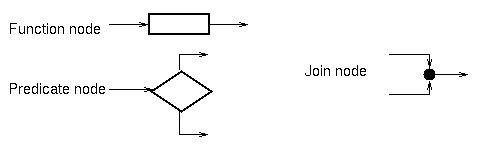
\includegraphics[width=\textwidth]{threeNodes}
\centering
\end{figure}

We define a \udef{proper program} as a flowchart which:
\begin{enumerate}
\item has a single entry arc;
\item has a single exit arc; and
\item has a path from the entry arc to each node and from each node to the exit arc.
\end{enumerate}

A \udef{prime program} is a proper program which has no embedded proper subprogram greater than one node. A sequence of function nodes is also considered prime.

A \udef{composite program} is a proper program that is not prime.

\begin{figure}[h]
\label{primeComposite}
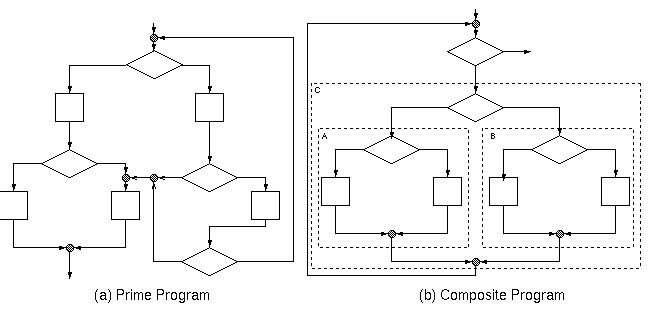
\includegraphics[width=\textwidth]{primeComposite}
\centering
\end{figure}

We can enumerate the prime programs. Figure \ref{primeEnumeration} describes all programs of up to $4$ nodes. 

\begin{figure}[h]
\label{primeEnumeration}
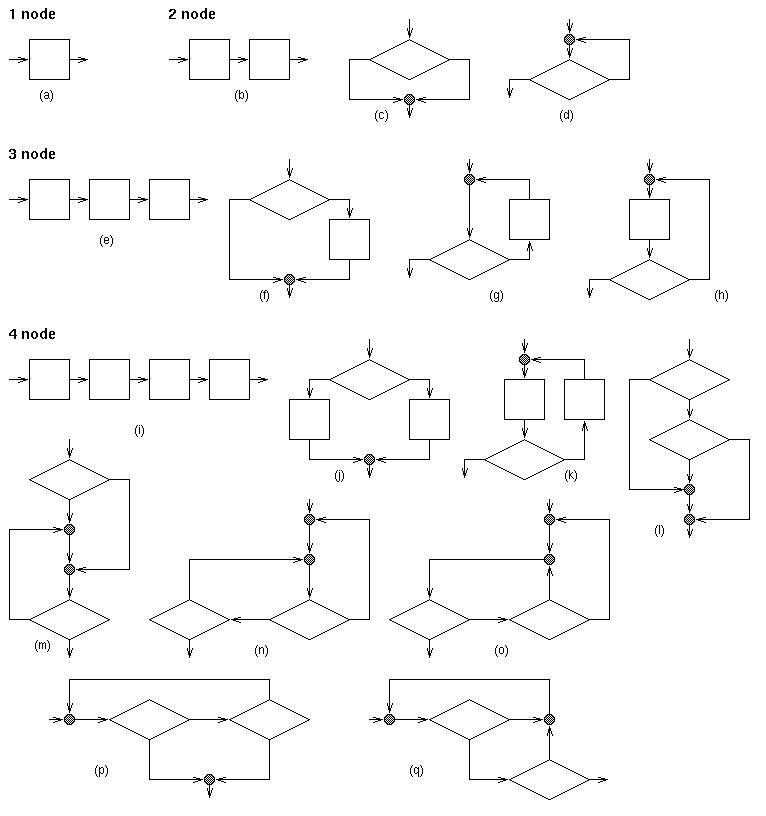
\includegraphics[width=\textwidth]{primeEnumeration}
\centering
\end{figure}

We can now classify these primes.
\begin{itemize}
\item Primes (a), (b), (e) and (i) represent sequences of function nodes.
\item Primes (c), (d), and (l) through (q) do not contain function nodes and thus do not change the state of the machine. They are either identity functions of or infinite loops.
\item The primes (f), (g), (h), (j) and (k) are the interesting primes. They represent the following control structures:
\item[(f)] is the \textbf{if-then},
\item[(g)] is the \textbf{while-loop},
\item[(h)] is the \textbf{do-while},
\item[(j)] is the \textbf{if-then-else} and
\item[(k)] is the \textbf{do-while-do}.
\end{itemize}
Most programming languages implement these control structures, except the do-while-do. This last structure has generally been ignored by language designers.

Other types of loops, such as for-loops can be considered syntactic sugar.
\subsubsection{Structured programming.}  
The goto statement is quite controversial. The paradigm of structured programming aims to improve clarity by eliminating goto statements and instead making use of the structured control flow constructs of selection (if/then/else) and repetition (while and for), block structures, and subroutines.

The goto statement has disadvantages:
\begin{enumerate}
\item The lack of hierarchical program structure can make programs less clear.
\item Making the order of statements in the program not necessarily the execution order can lead to confusion.
\item It violates the concept of \textit{one-in, one-out control structures}, making the design less understandable.
\item Groups of statements may serve multiple purposes. (On the other hand it can get rid of code duplication.)
\item It makes it hard to find a meaningful set of coordinates with which to describe the process progress. (See Dijkstra.)
\end{enumerate}


There are, however, also some advantages:
\begin{enumerate}
\item Direct hardware support. (This is relevant with poorly implemented Boolean variables and procedure calls, see in particular tail call optimization). TODO ref Knuth.
\item Simple and easy to use in small programs
\item Completely general purpose as a building block for simulating other control structures.
\item Some program structures are expressed more elegantly with a goto statement than with structures sequence control. Examples include:
\begin{itemize}
\item Loops with multiple natural exit points.
\item Simulating do-while-do loops.
\item Prematurely exiting a loop to deal with exceptional conditions.
\item When implementing state machines, state switches may conveniently be implemented using goto statements. This type of state-switching is often used in the Linux kernel.
\end{itemize}
In some languages these issues are addressed by using break statements, continue statements and throwing exceptions. All three of these however can be viewed as just a repackaging of the goto statement, with many of the same flaws.

Having said that, the practical consensus seems to be that these constructs are useful in practice.
\end{enumerate}

\subsubsection{Continuations}
First-class control
TODO?

\section{Subprogram control}
\subsection{Subprogram sequence control}
\subsubsection{Simple call-return.} In this view the main program may during execution call various subprograms, which may in turn call sub-subprograms. A very naive way to implement this is using the \textit{copy rule}: the code of the subprogram is simply copied into the main program whenever it is called.

Limitations of this naive view include the following:
\begin{enumerate}
\item \textit{Subprograms cannot be recursive.} A subprogram is \udef{directly recursive} if it calls itself at some point. A subprogram is \udef{indirectly recursive}	if it calls another subprogram that in turn calls the original subprogram.

If the copy rule were to be applied to a recursive subprogram, the resulting code would still call that subprogram. Thus we would be stuck in an infinite loop. This is problematic because recursion can be quite useful.

\item \textit{Subprograms must execute completely at each call.} Sometimes, however, we want the subprogram to resume execution from where it left off last time. This is essentially the idea behind coroutines.

\item \textit{Immediate transfer of control at point of call.} For a scheduled subprogram call we wish execution of the subprogram to be deferred until some later time.

\item \textit{Single execution sequence.} This implementation of subprograms does not support parallel programming.

\item \textit{Subprograms must be explicitly called.} Sometimes we do not know when we will want to call a subprogram. For instance an exception handler should be called whenever an exception is thrown. This is by definition exceptional.
\end{enumerate}

\paragraph{Implementation}
First we make a distinction between the \textit{definition} of a subprogram and its \textit{activation}. An activation record contains a reference to the code of the subprogram as well as an \textit{activation record} containing local data, parameters and other data.

Program flow is controlled by keeping track of pairs of pointers: The \udef{current-instruction pointer} (CIP) points to the statement currently being executed and the \udef{current-environment pointer} (CEP) points to the current activation record.

When a subprogram is called, the old CIP and CEP are stored somewhere. A new CIP is created pointing to the first statement of the code of the subprogram. A new CEP is created pointing to the newly created activation record.

When a subprogram ends, the old CIP and CEP are reinstated.

There are multiple ways the CIP and CEP may be stored. A stack may be used. Or they may be stored in the activation record of the new subprogram. If we only require the simple copy rule behaviour, we can even get away without the CEP: each subprogram can only ever have at most one activation record and thus we can statically allocate storage for a single activation record.

This simple model is often hardware-supported with a \textit{return-jump instruction}.

\subsubsection{Recursion.}
So long as both the CIP and CEP are stored, the implementation idea given above automatically supports recursion.

\subsubsection{Exceptions.} These are raised to signal exceptional circumstances, such as 
\begin{enumerate}
\item Error conditions
\item Unpredictable conditions
\item Tracing and monitoring
\end{enumerate}
An exception is typically propagated back up the call stack until the proper place th handle it.

The question of what to do once an exception has been handled does not have an obvious answer. Different languages have different solutions.
\paragraph{Assertions.} An assertion is a statement implying a relation among data in a program. During testing it will typically raise an error if that relation is violated. After testing it may remain as documentation. See also design by contract.

\subsubsection{Scheduling.} Scheduling can take several different forms, such as
\begin{enumerate}
\item Schedule subprograms to execute before or after other subprograms.
\item Schedule subprograms the be executed when a Boolean expression becomes true.
\item Schedule the execution of subprograms based on time.
\item Schedule subprograms based on priority.
\end{enumerate}

\subsubsection{Coroutines}. Coroutines are subprograms that can exit before completing execution. When it is called again, it resumes from where it left off. Two coroutines can pass control between themselves.

\subsubsection{Generators}. Generators, also known as semicoroutines, are like coroutines, but lack a coroutines ability to specify where it yields control to. It is still possible to implement coroutines on top of a generator facility, with the aid of a top-level dispatcher routine.

\subsubsection{Parallel programming}
TODO: move to separate section?
\paragraph{Things to take into account.} Parallel programming constructs add complexity to the language design. The following topics must be adressed.
\begin{enumerate}
\item \textit{Variable definitions.} If variables are mutable, we can run into synchronization problems. Definitional (i.e. immutable) variables do not have this problem.
\item \textit{Parallel composition.} We need ways to fork program execution and create additional threads of control.
\item \textit{Program structure}. Parallel programs generally follow one of two execution models:
\begin{enumerate}
\item They may be transformational, where the goal is to transform the input data into an appropriate output value. Parallelism is applied to speed up the process.
\item They may be reactive where the program reacts to external stimuli, called events.
\end{enumerate}
\item \textit{Communication} between parallel programs may happen through the use of shared memory or via messages.
\end{enumerate}
\paragraph{And or fork statements}
With this statement we can designate parts of the program that we can allow to be executed at the same time.

\paragraph{Guarded commands} These were proposed in the 1970s by Dijkstra. They provide a way to write nondeterministic programs.

A guarded statement has a condition, called a \udef{guard}, such that the statement is not executed if the guard is false. We consider the following types of guarded statements:
\begin{itemize}
\item The \textbf{guarded if statement} contains several guarded statements. At least one for the guards must be true. If multiple guards are true, the statement to execute is chosen nondeterministically.
\item The \textbf{guarded repetition statement} is like the guarded if statement that repeats as long as some guard is true.
\end{itemize}
TODO: move?? Also expand.

\paragraph{Tasks} Ordinarily when a subprogram is called, execution of the main program is suspended. If the subprogram is called as a task, the execution of the main program continues.

Task management can obviously be non trivial. In order for tasks running asynchronously to coordinate their activities, the language must provide some means of synchronization. This may be achieved in several ways:
\begin{enumerate}
\item \textbf{Interrupts}. If task A wishes to signal to task B that a particular event has occurred, then task A executes an instruction that causes the execution of task B to be interrupted immediately. Control is then handed to a subprogram or section of code that handles the interrupt. Afterwards control is handed back to task B.

This is a mechanism commonly found in computer hardware. It is also similar to exception handling. In high level-languages, interrupts have several disadvantages:
\begin{enumerate}
\item The code for interrupt handling is separate from the main body of the task, leading to a more confusing program structure.
\item A task waiting for an interrupt must usually enter a busy waiting loop.
\item The task must be written so that an interrupt can be handled at any time.
\end{enumerate}
\item \textbf{Semaphores}. TODO. A semaphore is a data object consisting of two parts:
\begin{enumerate}
\item An integer counter. In a binary semaphore this counter may only be one or zero, in a general semaphore it may be any non-negative integer.
\item A queue of tasks.
\end{enumerate}
Two operations are defined for a semaphore data object $P$:
\begin{enumerate}
\item \texttt{signal(P)}. When executed by a task A, this operation tests the value of the counter in $P$. If zero, the first task in the task queue is removed from the queue and executed. If not zero, or if the queue is empty, the counter is incremented by one. Execution of task A continues after the signal operation is complete.
\item \texttt{wait(P)}. When executed by task B, this operation tests the value of the counter in $P$. If nonzero, the counter is decremented by one and task B continues execution. If zero, task B is inserted at the end of the task queue for $P$ and the execution of B is suspended.
\end{enumerate}
Semaphores have some disadvantages for use in high-level languages:
\begin{enumerate}
\item A task can only wait for one semaphore at a time.
\item If a task fails to signal, the system of tasks may deadlock.
\item Programs with several tasks and semaphores become increasingly difficult to understand, debug and verify.
\item All tasks accessing the semaphore must share memory.
\end{enumerate}
\item \textbf{Messages} can be passed between tasks. The basic concept is similar to a pipe. Implementations of this system can be quite complex. Several tasks may simultaneously try to send messages. The implementation must then provide some way to store those messages until the receiver can process them.
\item \textbf{Guarded commands.} See above.
\item \textbf{Rendezvous.} Used in Ada. Like messages, but must be accepted.
\end{enumerate} 

\subsection{Shared data in subprograms}
Data can either be shared directly, using parameters, or indirectly by giving the subprogram access to nonlocal environments.

\subsubsection{Parameters and parameter transmission}
A \udef{(formal) parameter} is a variable declared in the function definition, that must be given some data when the function is called. This data that is given to the function is called an \udef{argument} or \udef{actual parameter}.

There are multiple ways to specify which argument should go to which parameter. This can, e.g., be done through positional correspondence or by explicitly naming the parameter.

There are also multiple ways to transmit parameters. Depending on the method of transmission, parameters can also be used to return data from the subprogram. In most languages a single value may also be returned as an explicit function value.

In some languages the distinction is made between between function calls with a return value and procedure or subroutine calls without a return value.

\paragraph{Call by name.} In this model the actual parameter is substituted everywhere for the formal parameter. This results in overhead leads to complications.
\paragraph{Call by reference.} A pointer to the location of the data object is made available to the subprogram.
\paragraph{Call by value.} The value of the argument is copied into a variable with the name of the formal parameter.
\paragraph{Call by value-result.} Like call by value, except at the end of the subprogram the contents of the local variable is copied back into the original argument variable.
\paragraph{Call by constant value.} The formal argument acts like a local constant.
\paragraph{Call by result.} This parameter is only used to transmit a result back from a subprogram. 

\subsubsection{Data sharing through environments.}
TODO
\paragraph{Explicit common environments.}
TODO

\subsection{First-class subprograms}
If we say a language has first-class subprograms or functions, it means functions are treated just like any other data type. TODO

\subsubsection{Closures}
TODO

\subsection{Factors that obscure the definition of subprograms as mathematical functions}
\begin{enumerate}
\item Implicit arguments.
\item Implicit results (side-effects).
\item Behaviour can be undefined for some arguments. In general the domain is too broad and needs to be narrowed with conditional statements.
\item History sensitive.
\end{enumerate}

\subsection{Tail call optimization}
TODO


\section{Miscellaneous language features}
TODO Reflection


\section{Tools}
\subsection{ANTLR}
\subsection{YACC - LEX / BISON}
\subsection{LLVM}
Also JVM, GCC?
\subsection{Racket}


\chapter{Paradigms and patterns}
\section{The object-oriented paradigm}
\subsection{Encapsulation}
\subsection{Inheritance}
\subsection{Polymorphism}

\section{Design patterns}
Observer, Decorator, Factory, Singleton, Command, Adapter, Facade, Template method, Iterator, Composite, State, Proxy, Compound patterns

Bridge, Builder, Chain of responsability, Flyweight, Interpreter, Mediator, Memento, Prototype, Visitor

Visitor, listener, module
\subsection{Dynamic languages}
\subsubsection{Monkey patching}

\chapter{Practical coding}
code smell

readability (clarity)

Magic numbers

SOLID, STUPID

DRY

Object calisthenics:
\begin{enumerate}
\item Only one level of indentation per method
\item Do not use else
\item Wrap primitive types (especially if they contain behavior)
\item Only one method call per line.
\item Do not abbreviate
\item Keep classes small: about 10 methods of 10 lines each.
\item Limit your instance variables to two.
\item Use first class collections
\item Don't use getters and setters. Too generic.
\end{enumerate}

\section{Development processess}
\subsection{Iterative and waterfall processes}
The essential difference is how a project gets broken up into smaller chunks. To build software you might have to do certain activities: requirements analysis, design, coding and testing.

\begin{itemize}
\item The \udef{waterfall} style breaks down the project based on those activities, e.g. having 2-month analysis, 4-month design, 3-month coding and 3-month testing phases.
\item The \udef{iterative} styles breaks down a project by subsets of functionality. This means performing all four activities so you have a systems that works well with only a part of the functionality, then performing all four activities again to add more functionality. And again, and again.

A common technique is \udef{time boxing} where the scope of each iteration is determined by time, not feature set.

At the end of each iteration an \textbf{iteration retrospective} may be held. A good way to do this is to make a list with three categories:
\begin{itemize}
\item \textit{Keep:} things that worked well that you want to ensure you continue to do.
\item \textit{Problems:} areas that aren't working well.
\item \textit{Try:} changes to your process to improve it.
\end{itemize}
\end{itemize}

In practice, of course, there is some overlap. With waterfall development there are often backflows: during coding and testing it may be necessary to revisit analysis and design. These backflows should be minimised as much as possible.

With iteration there is usually some form of exploration activity and analysis before the true iteration begins. At the end there is usually a global stabilisation period to iron out bugs. Also other activities, such as user training, may not be part of the iteration.

There are also hybrid processes, such as first doing analysis and high-level design in waterfall style and then dividing coding and testing into iterations.

\begin{params}
Many people agree pure waterfall is bad, but it is still most common in industry. Often people claim to be working iteratively when in fact they doing waterfall. Common symptoms include
\begin{itemize}
\item ``We are doing one analysis iteration followed by two design iterations.''
\item ``This iteration's code is very buggy, but we'll clean it up at the end.''
\end{itemize}
\end{params}

TODO: rework.
The iterative approach explicitly assumes that existing code will be reworked and deleted. This process can be made more efficient with
\begin{itemize}
\item Automated regression testing
\item Refactoring
\item Continuous integration
\end{itemize}

\subsection{Predictive and adaptive planning}
With \udef{predictive planning} a project has two phases. The first is coming up with plans and is difficult to predict, but the second is much more predictable because the plans are in place. 

The problem is that often requirements change. This is called \udef{requirements churn}. To combat this you could spend more time planning, but often requirements churn is unavoidable. In such cases one needs to settle for \udef{adaptive planning}, where everything is constantly reevaluated.

\subsection{Agile processes}
The Manifesto for Agile Software Development (\url{https://agilemanifesto.org/}) states the following values:
\begin{displayquote}
{\Large Individuals and interactions} over processes and tools \\
{\Large Working software} over comprehensive documentation \\
{\Large Customer collaboration} over contract negotiation \\
{\Large Responding to change} over following a plan
\end{displayquote}
As well as the following principles:
\begin{displayquote}
\begin{enumerate}
\item Our highest priority is to satisfy the customer
through early and continuous delivery
of valuable software.
\item Welcome changing requirements, even late in
development. Agile processes harness change for
the customer's competitive advantage.
\item Deliver working software frequently, from a
couple of weeks to a couple of months, with a
preference to the shorter timescale.
\item Business people and developers must work
together daily throughout the project.
\item Build projects around motivated individuals.
Give them the environment and support they need,
and trust them to get the job done.
\item The most efficient and effective method of
conveying information to and within a development
team is face-to-face conversation.
\item Working software is the primary measure of progress.
\item Agile processes promote sustainable development.
The sponsors, developers, and users should be able
to maintain a constant pace indefinitely.
\item Continuous attention to technical excellence
and good design enhances agility.
\item Simplicity -- the art of maximizing the amount
of work not done -- is essential.
\item The best architectures, requirements, and designs
emerge from self-organizing teams.
\item At regular intervals, the team reflects on how
to become more effective, then tunes and adjusts
its behavior accordingly.
\end{enumerate}
\end{displayquote}

Agile processes are strongly adaptive and very much people-oriented. They also tend to use short, time-boxed iterations with little weight attached to documents and ceremony. For this reason they are often characterised as \textbf{lightweight} (this is a consequence of adaptivity and people orientation).
\subsubsection{Extreme programming (XP)}
\subsubsection{Scrum}
\subsubsection{Feature driven development (FDD)}
\subsubsection{Crystal}
\subsubsection{Dynamic systems development method (DSDM)}

\subsection{Rational unified processes (RUP)}
RUP is a project framework: the first step is to choose a development case, i.e. the process used in the project.

All RUP projects follow four phases:
\begin{itemize}
\item Inception
\item Elaboration
\item Construction
\item Transition
\end{itemize}
RUP is only compatible with an iterative work flow.

\section{Design documents and documentation}
Detailed documentation generated from the code and external documentation. External documentation should be comprehensible, not comprehensive.

Document design alternatives that were not chosen and why not.

\section{Coding styles}
defensive, total, 
design by contract
\section{Testing}
Difference in style
\subsection{Unit testing}
\section{Coding in a team}
I have very little experience with this. This section is mostly just a place for me to put tips I have heard for future reference.

\section{Version control}
\subsection{Git}
\subsection{Subversion}

\section{Benchmarking}
\section{Optimization}
Precompute (integral pictures)

Only worry about bottlenecks. Premature optimization is the root of all evil.

Inner loops

Timing analysis

\chapter{Notes on selected languages}
\addtocontents{toc}{\protect\setcounter{tocdepth}{2}}
\section{History}
Here an attempt will be made to very briefly highlight some of the ideas, features and syntax of a number of languages. The classification is quite arbitrary as most languages support multiple paradigms.
\section{Assembly languages}
RISC >< CISC
\subsection{M32}
\subsection{Z80}
\subsection{(M)MIX}
\subsection{x86}
\subsection{ARM}

\section{Procedural languages}
\subsection{FORTRAN 77}
\paragraph{History.}
FORTRAN (FORmula TRANslation) was the first high-level programming language to become widely used. At conception, in 1957, there were serious concerns as to whether a high-level language could ever seriously compete with assembly languages. Thus design was oriented heavily towards efficiency.

The language went through many revisions. The biggest change was between FORTRAN 77 and Fortran 90. Fortran 95 is the most widely implemented of the more recent specifications and later versions are largely similar.

\paragraph{Syntactic features.}
The basic structure of a program can be seen in this hello world example.
\begin{lstlisting}[language={[77]fortran}, style=program]
      program helloworld
        print *, "Hello world!"
        stop
        end
\end{lstlisting}
The \texttt{stop} statement is optional since the program will stop when it reaches the end, but is recommended to emphasize that execution flow stops there. You cannot have a variable with the same name as the program.

FORTRAN is completely case insensitive and was traditionally written in all caps. Current practice is to mix upper and lower case.

Blanks are ignored completely, in fact they may all be removed. Spaces may be inserted freely.

FORTRAN 77 uses fixed-format source code:
\begin{itemize}
\item Comments must begin with a \texttt{C} or a \texttt{*} in column 1. Some compilers allow in-line comment with an \texttt{!}. The exclamation mark may appear anywhere on a line, except in positions 2-6.
\item Statement labels must occur in columns 1-5
\item Continuation lines must have a non-blank character in column 6. Any non-blank character can be used as a continuation character. Traditionally a plus, an ampersand or a digit is used. Example:
\begin{lstlisting}[language={[77]fortran}, style=snippet]
c The next statement goes over two physical lines
      area = 3.14159265358979
     +       * r * r
\end{lstlisting}
\item Statements must start in column 7.
\item The line-length may be limited to 72 characters (derived from the 80-byte width of a punch-card, with last 8 characters reserved for (optional) sequence numbers)
\end{itemize}



\subparagraph{Variables, types and declarations}
Variables are 1 to 6 characters long, begin with a letter and may contain letters and digits.

Reserved words are: \texttt{assign, backspace, block data, call, close, common, continue, data, dimension, do, else, else if, end, endfile, endif, entry, equivalence, external, format, function, goto, if, implicit, inquire, intrinsic, open, parameter, pause, print, program, read, return, rewind, rewrite, save, stop, subroutine, then, write}.

Variables do not have to be explicitly declared. Explicit declarations take the form
\begin{lstlisting}[language={[77]fortran}, style=snippet]
      integer A, B, C
      real radius, eulerE
      double precision q, r
      complex z
      logical t
      character ch
\end{lstlisting}
If there is no explicit declaration, a \textit{naming convention} is used. By default variable names beginning with \texttt{I-N} are integer variables; all others are real. This default behaviour can be modified with an \texttt{IMPLICIT} statement:
\begin{lstlisting}[language={[77]fortran}, style=snippet]
      IMPLICIT INTEGER (A-Z)
\end{lstlisting}
This causes the type integer to be assumed for all variables.

Constants are defined in the following way
\begin{lstlisting}[language={[77]fortran}, style=snippet]
      PARAMETER (KMAX = 100, MIDPT = 50)
\end{lstlisting}
the \texttt{parameter} statement(s) must come before the first executable statement.

\subparagraph{Arrays.} One-dimensional arrays are declared as follows.
\begin{lstlisting}[language={[77]fortran}, style=snippet]
      real a(20)
      real b(0:19), weird(-162:237)
      double precision x(100)
\end{lstlisting}
By default arrays are indexed from $1$ to their length, inclusive. Arbitrary index ranges can also be defined, see arrays \texttt{b} and \texttt{wierd} above.

Elements or arrays can be accessed using brackets: \texttt{a(3) = 2.0}. The Fortran compiler does not check whether array elements are out of bounds or undefined!

Multi-dimensional arrays can be declared in a similar way by putting a comma between indexes:
\begin{lstlisting}[language={[77]fortran}, style=snippet]
      real A(3,5,2:7)
      A(1,4,2) = 5
\end{lstlisting}

Two-dimensional arrays are stored in memory as contiguous sequences of elements, column by column.

An alternative (old-fashioned) style is to use the \texttt{dimension} statement:
\begin{lstlisting}[language={[77]fortran}, style=snippet]
      real A, x
      dimension x(50)
      dimension A(10,20)
C This is equivalent to:
      real A(10,20), x(50)
\end{lstlisting}

\subparagraph{The \texttt{DATA} statement} is a compact way to input data that is known at compile time. The syntax is as follows
\begin{lstlisting}[language={[77]fortran}, style=snippet]
      data m/10/, n/20/, x/2.5/, y/2.5/
C Or alternatively
      data m,n/10,20/, x,y/2*2.5/
\end{lstlisting}
Both statements result in \texttt{m = 10, n = 20, x = 2.5, y = 2.5}.

The data statement is performed only once, right before the execution of the program starts. For this reason, the data statement is mainly used in the main program and not in subroutines. It can also be used to initialize arrays (vectors, matrices).
\begin{lstlisting}[language={[77]fortran}, style=snippet]
      real A(10,20)
      data A/ 200 * 0.0/
C Individual elements may also be initialised
      data A(1,1)/ 12.5/, A(2,1)/ -33.3/, A(2,2)/ 1.0/
\end{lstlisting}

The data statement cannot be used for variables contained in a common block. There is a special syntax for this purpose, called \texttt{block data}.
\begin{lstlisting}[language={[77]fortran}, style=snippet]
      block data
        integer nmax
        parameter (nmax=20)
        real v(nmax), alpha, beta
        common /vector/v,alpha,beta
        data v/20*100.0/, alpha/3.14/, beta/2.71/
      end
\end{lstlisting}

The block data may not be nested inside the main program or a subroutine.

\paragraph{Expressions and assignment}
FORTRAN supports the following literals:
\begin{itemize}
\item Integer literals
\begin{lstlisting}[language={[77]fortran}, style=snippet]
      1
      0
      -100
      32767
      +15
\end{lstlisting}
\item Real literals
\begin{lstlisting}[language={[77]fortran}, style=snippet]
      1.0
      -0.25
      2.6E6
      3.333E-1
\end{lstlisting}
The $E$ means multiply by $10$ to the power of whatever comes after it.
\item Double precision literals
\begin{lstlisting}[language={[77]fortran}, style=snippet]
      2.0D-1
      1D99
\end{lstlisting}
Like reals, but $D$ instead of $E$.
\item Complex literals
\begin{lstlisting}[language={[77]fortran}, style=snippet]
      (2, -3)
      (1., 9.9E-1)
\end{lstlisting}
\item Logical literals
\begin{lstlisting}[language={[77]fortran}, style=snippet]
      .TRUE.
      .FALSE.
\end{lstlisting}
\item Character literals. Most often used in arrays (as strings). Some versions of FORTRAN require single quotes.  An enclosed single-quote can be represented by doubling.
\begin{lstlisting}[language={[77]fortran}, style=snippet]
      'ABC'
      'Anything goes!'
      'It''s a nice day'
\end{lstlisting}
\end{itemize}

Operator precedence in FORTRAN 77 (from highest to lowest):
\begin{enumerate}
\item[\texttt{**}] Exponentiation
\item[\texttt{-}] Unary minus
\item[\texttt{*, /}] Multiplication, division
\item[\texttt{+,-}] Addition, subtraction
\item[] Relational operators: \texttt{.LT., .LE., .GT., .GE., .EQ., .NE.} (respectively $<, <=, >, >=, =, \backslash=$).
\item[\texttt{.NOT.}] Logical not
\item[\texttt{.AND.}] Logical and
\item[\texttt{.OR.}] Logical or
\end{enumerate}
For different evaluation order, use parentheses.

Caution must be taken when using the \undline{division operator}. If both operands are integer, integer division is performed, otherwise real arithmetic division is performed.

Assignment is done with the equals sign
\begin{lstlisting}[language={[77]fortran}, style=snippet]
      area = pi * r**2
\end{lstlisting}

For type conversion, the following functions are available: \texttt{int(), real(), dble(), ichar(), char()}. The function \texttt{ichar} converts a character into an integer; \texttt{char} does the opposite.

Constructs that are not statically checked are ordinarily left unchecked.

\paragraph{Flow control.}
The \texttt{if} statement comes in several forms:
\begin{lstlisting}[language={[77]fortran}, style=snippet]
      if (x .LT. 0) x = -x
\end{lstlisting}
or
\begin{lstlisting}[language={[77]fortran}, style=snippet]
      if (x .LT. 0) then
        x = -x
      endif
\end{lstlisting}
or
\begin{lstlisting}[language={[77]fortran}, style=snippet]
      if (x .LT. 0) then
        x = -x
      elseif (x .GT. 5) then
        x = 5
      else
        x = x+1
      endif
\end{lstlisting}
\texttt{if} statements can also be nested.

FORTRAN 77 only has the \texttt{do}-loop. An example:
\begin{lstlisting}[language={[77]fortran}, style=snippet]
      integer i, n, sum
 
      sum = 0
      do 10 i = 1, n
         sum = sum + i
         write(*,*) 'i =', i
         write(*,*) 'sum =', sum
  10  continue
\end{lstlisting}
Here the number $10$ is a label. Column positions 1-5 are reserved for statement labels. Typically, most programmers use consecutive multiples of 10.

The \texttt{continue} statement is a placeholder that does nothing.

The statement identified by the label after the \texttt{DO} command is called the \udef{terminal statement}.

The variable is typically incremented by one each loop until the second value is reached (inclusive). A step may also be specified (negative means counting down).
\begin{lstlisting}[language={[77]fortran}, style=snippet]
      integer i
 
      do 20 i = 10, 1, -2
         write(*,*) 'i =', i
  20  continue
\end{lstlisting}

Many compilers also allow the \texttt{DO} statement to be closed by \texttt{ENDDO}. This is not ANSI FORTRAN 77, however. The expressions in the beginning of the \texttt{DO}-loop arwe evaluated only once. So the following loop does not run forever:
\begin{lstlisting}[language={[77]fortran}, style=snippet]
      integer i,j
 
      read (*,*) j
      do 20 i = 1, j
         j = j + 1
  20  continue
      write (*,*) j
\end{lstlisting}

Other types of loops have to be simulated using \texttt{GOTO} statements.
\begin{lstlisting}[language={[77]fortran}, style=snippet]
     integer n

     n = 1
  10 if (n .LE. 100) then
        write (*,*) n
        n = 2*n
        goto 10
     endif
\end{lstlisting}

\paragraph{Subprograms.}
Fortran has two different types of subprograms, called functions and subroutines. 

Functions take a set of input arguments (parameters) and return a value of some type.
Some built-in functions include:
\begin{lstlisting}
abs     absolute value
min     minimum value
max     maximum value
sqrt    square root
sin     sine
cos     cosine
tan     tangent
atan    arctangent
exp     exponential (natural)
log     logarithm (natural)
\end{lstlisting}

An example of a user-defined function:
\begin{lstlisting}[language={[77]fortran}, style=snippet]
      real function r(m,t)
        integer m
        real t
        r = 0.1*t * (m**2 + 14*m + 46)
        if (r .LT. 0) r = 0.0
        return
      end
\end{lstlisting}
We see
\begin{itemize}
\item Functions have a type. If none is declared, the same implicit typing system as for variables is used.
\item Functions are terminated by the \texttt{return} statement.
\item The return value should be stored in a variable with the same name as the function. 
\item Strictly speaking Fortran 77 does not permit recursion. However, it is not uncommon for a compiler to allow recursion. 
\end{itemize}

A subroutine does not return a value. The syntax is as follows:
\begin{lstlisting}[language={[77]fortran}, style=snippet]
      subroutine iswap (a, b)
        integer a, b
        integer tmp
        tmp = a
        a = b
        b = tmp
        return
      end
\end{lstlisting}
The subroutine works because parameters in FORTRAN 77 subprograms are \undline{passed by reference.}

We can pass arrays of arbitrary size to subprograms if we define the arrays in the subprogram with dummy indices (usually an asterisk).

\paragraph{Common blocks and scope.}
FORTRAN 77 has no global variables. Common blocks can be used instead. In general the syntax is as follows
\begin{lstlisting}[language={[77]fortran}, style=snippet]
      program main
        real alpha, beta
        common /coeff/ alpha, beta
        [ statements ]
        stop
      end
C
      subroutine sub1 ( [ some arguments ] )
        [ declarations of arguments ]
        real alpha, beta
        common /coeff/ alpha, beta
        [ statements ]
        return
      end
C
      subroutine sub2 ( [ some arguments ] )
        [ declarations of arguments ]
        real alpha, beta
        common /coeff/ alpha, beta
        [ statements ]
        return
      end
\end{lstlisting}
The syntax of a common statement is: \texttt{COMMON / name / list-of-variables}. A variable cannot belong to more than one common block. The variables in a common block do not need to have the same names each place they occur (although it is a good idea to do so), but they must be listed in the same order and have the same type and size.

Putting arrays in common blocks is a bad idea.
\paragraph{I/O.} In FORTRAN each file is associated with a unit number, an integer between 1 and 99. Some unit numbers are reserved: 5 is standard input, 6 is standard output. 

Before you can use a file you have to open it. The command is 
\begin{lstlisting}[language={[77]fortran}, style=snippet]
      open (list-of-specifiers)
\end{lstlisting}
Where the most common specifiers are
\begin{lstlisting}
[UNIT=]  u
IOSTAT=  ios
ERR=     err
FILE=    fname
STATUS=  sta
ACCESS=  acc
FORM=    frm
RECL=    rl
\end{lstlisting}
\begin{itemize}
\item[\texttt{u}]  is a number between 1 and 99 inclusive that denotes the file.
\item[\texttt{ios}] is the I/O status identifier and should be an integer variable. Upon return, \texttt{ios} is set to zero if the statement was successful and set to a non-zero value otherwise. 
\item[\texttt{err}] is a label which the program will jump to if there is an error. 
\item[\texttt{fname}] is a character string denoting the file name. 
\item[\texttt{sta}] is a character string that has to be either \texttt{NEW}, \texttt{OLD} or \texttt{SCRATCH}. It shows the prior status of the file. A scratch file is a file that is created when opened and deleted when closed (or the program ends). 
\item[\texttt{acc}] must be either \texttt{SEQUENTIAL} or \texttt{DIRECT}. The default is \texttt{SEQUENTIAL}.
\item[\texttt{frm}] must be either \texttt{FORMATTED} or \texttt{UNFORMATTED}. The default is \texttt{UNFORMATTED}. 
\item[\texttt{rl}] specifies the length of each record in a direct-access file. 
\end{itemize}
After a file has been opened, you can access it by read and write statements. When you are done with the file, it should be closed by the statement 
\begin{lstlisting}[language={[77]fortran}, style=snippet]
      close ([UNIT=]u[,IOSTAT=ios,ERR=err,STATUS=sta])
\end{lstlisting}
In this case \texttt{sta} is a character string which can be \texttt{KEEP} (the default) or \texttt{DELETE}. 

Reading and writing is done as follows:
\begin{lstlisting}[language={[77]fortran}, style=snippet]
read ([UNIT=]u, [FMT=]fmt, IOSTAT=ios, ERR=err, END=s) [ list-of-variables ]
write([UNIT=]u, [FMT=]fmt, IOSTAT=ios, ERR=err, END=s) [ list-of-variables ]
\end{lstlisting}
The \texttt{END=s} specifier defines which statement label the program jumps to if it reaches end-of-file. The format number \texttt{fmt} refers to a label for a format statement (described below).

The first two arguments can be replaced with asterisks. This is sometimes called \udef{list directed} read / write. This format assumes the file has a line per record and the fields are separated by blanks or commas.

If we are reading or writing to the stantard input, the followinf syntax may be used (the asterisk refers to the format):
\begin{lstlisting}[language={[77]fortran}, style=snippet]
      read  *, [ list-of-variables ]
      print *, [ list-of-variables ]
\end{lstlisting}

\paragraph{The \texttt{FORMAT} statement} TODO

\paragraph{Language design notes}

Changes compared to FORTRAN 66:
\begin{itemize}
\item Additions:
\begin{itemize}
\item Block \texttt{IF} and \texttt{END IF} statements, with optional \texttt{ELSE} and \texttt{ELSE IF}.
\item \texttt{DO}-loop extensions including
\begin{itemize}
\item parameter expressions
\item negative increments
\item zero trip counts
\item Better file I/O.
\item The \texttt{IMPLICIT} statement.
\item The \texttt{PARAMETER} statement.
\item The \texttt{CHARACTER} datatype.
\item Lexical comparison of strings with \texttt{LGE, LGT, LLE, LLT}.
\end{itemize}
\end{itemize}
\item Deprecated:
\begin{itemize}
\item Hollerith constants and Hollerith data.
\item Transfer of control out of and back into the range of a DO loop (also known as "Extended Range")
\end{itemize}
\end{itemize}
\subsection{Fortran 95}
Changes compared to Fortran 90:
\begin{itemize}
\item Additions:
\begin{itemize}
\item 
\end{itemize}
\item Deprecated:
\begin{itemize}
\item
\end{itemize}
\item Changes:
\begin{itemize}
\item 
\end{itemize}
\end{itemize}
Changes in FORTRAN 2003:
\begin{itemize}
\item Additions:
\begin{itemize}
\item 
\end{itemize}
\item Deprecated:
\begin{itemize}
\item
\end{itemize}
\item Changes:
\begin{itemize}
\item 
\end{itemize}
\end{itemize}
Changes in FORTRAN 2008:
\begin{itemize}
\item Additions:
\begin{itemize}
\item 
\end{itemize}
\item Deprecated:
\begin{itemize}
\item
\end{itemize}
\item Changes:
\begin{itemize}
\item 
\end{itemize}
\end{itemize}
Changes in FORTRAN 2018:
\begin{itemize}
\item Additions:
\begin{itemize}
\item 
\end{itemize}
\item Deprecated:
\begin{itemize}
\item
\end{itemize}
\item Changes:
\begin{itemize}
\item 
\end{itemize}
\end{itemize}
\subsection{C}
\subsection{Pascal}
Of course, in stupid languages like Pascal, where labels cannot be
descriptive, GOTOs can be bad. But that's not the fault of the goto,
that's the braindamage of the language designer.


\subsection{SNOBOL}
\subsubsection{History}
Development of SNOBOL (StriNg Oriented and symBOlic Language) began in 1962 at AT\&T Bell Labs by Ralph Griswold, Ivan Polonsky and David Farber. The goal was to develop a string processing language for formula manipulation and graph analysis. The most successful version was SNOBOL4, developed in the 1970s.

SPITBOL (Speedy Implementation of SNOBOL) is a compiled implementation of the SNOBOL4.
\subsubsection{Concepts}
\begin{itemize}
\item Pattern matching language based upon BNF Grammars.
\item Patterns are a first-class data type.
\end{itemize}
\subsection{Go}

\section{UML}
\subsection{What is it?}
The Unified Modeling Language (UML) is a family of graphical notations that help describing and designing software systems, particularly software systems built using the object-oriented paradigm. The UML is a relatively open standard, controlled by the Object Management Group (OMG), an open consortium of companies. The UML was born out of the unification of many graphical modeling languages around in the late 1980s and early 1990s.

\subsubsection{Ways of using it}
One can identify three modes in which UML is often used:
\begin{enumerate}
\item \textbf{UML as a sketch.} In this usage UML is used to communicate some aspect of a system. Such a sketch is by no means complete, but just meant to illustrate an idea. Selectivity is key.
\item \textbf{UML as a blueprint.} In this usage the UML diagram is meant to be a complete and detailed guide to the code. A blueprint may be of the whole system or of a particular area. Such diagrams can be used by specialised \udef{CASE (computer aided software engineering) tools}.
\item \textbf{UML as a programming language} is when the blueprint is complete and accurate enough that it can mechanically be converted into executable code. The standard approach is called \udef{Model-Driven Architecture (MDA)}. 
\end{enumerate}

The UML can also be used for conceptual modeling or software modeling.
\begin{enumerate}
\item In the \textbf{software perspective}, the UML elements map (fairly) directly to elements in the software system. Within the software perspective, a distinction can also be made between diagrams focusing on \textit{interface} or \textit{implementation}.
\item In the \textbf{conceptual perspective}, the diagram deals in concepts, not necessarily actual components in the system.
\end{enumerate}

The UML standard can also be seen as having either \textit{prescriptive} or \textit{descriptive} rules. TODO Fowler p.13

\subsubsection{Notation and meta-model}
The UML defines
\begin{itemize}
\item a \textbf{notation} (i.e. graphical syntax) and
\item a \textbf{meta-model} which defines the concepts of the language.
\end{itemize}
When referring to the UML, sometimes the notation and sometimes the meta-model is meant.

\subsubsection{UML diagrams}

\subsection{Class diagrams}
\begin{wrapfigure}{r}{0.3\textwidth}
\vspace{-10pt}
\begin{tikzpicture}
\umlclass{Order}{
  dateReceived : Date[0..1] \\ isPrepaid: Boolean[1] \\ number: String[1] \\ price: Money
}{dispatch \\ close}
\end{tikzpicture}
\vspace{-20pt}
\end{wrapfigure}

A class diagram describes the various types of objects in the system and the static relationships that exist among them. Each class has a name and several \udef{features}, i.e. the properties and operations of a class. 

\subsubsection{Properties}
\udef{Properties} represent the structural features of a class. Properties appear in two very distinct notations: \textit{attributes} and \textit{associations}.

\paragraph{Attributes} define the property within the class box itself. They are put in the section under the title. The full form of an attribute is:
\begin{syntax}
\opt{\textit{visibility}} \opt{/} \textit{name} \opt{: \textit{type}} \opt{[\textit{multiplicity}]} \opt{= \textit{default}} \opt{\textit{property-string}}
\end{syntax}
Only \texttt{\textit{name}} is necessary.
\begin{itemize}
\item \texttt{\textit{visibility}} can be
\begin{itemize}
\item \texttt{+} for public
\item \texttt{-} for private
\item \texttt{$\sim$} for package
\item \texttt{\#} for protected
\end{itemize}
\item \texttt{/} means the property is a derived property, i.e. calculated from other properties.
\item \texttt{\textit{name}} is the name of the attribute.
\item \texttt{\textit{type}} indicates what kind of object may be placed in the attribute.
\item \texttt{\textit{multiplicity}} shows how many objects may fill the property. Multiplicities may be specified as
\begin{itemize}
\item \texttt{\textit{number}}: the property contains \texttt{\textit{number}} objects.
\item \texttt{\textit{lowerBound}..\textit{upperBound}}: the property contains more than \texttt{\textit{lowerBound}}, but no more than \texttt{\textit{upperBound}}, objects.
\item \texttt{*}: the property contains an arbitrary number (zero or more) of objects.
\item \texttt{\textit{lowerBound}..*}: the property contains more than \texttt{\textit{lowerBound}} objects.
\end{itemize}
\item \texttt{\textit{number}} is the value for a newly created object if the attribute is not specified during creation.
\item \texttt{\textit{property-string}} is of the form
\begin{syntax}
\{ \textit{property-modifier} \mult{, \textit{property-modifier}} \}
\end{syntax}
where \texttt{\textit{property-modifier}} can be one of
\begin{itemize}
\item \texttt{id}: the property is part of the identifier for the class which owns the property.
\item \texttt{readOnly}: clients may not modify the property.
\item \texttt{ordered} or \texttt{unordered}: the objects associated with this multi-valued property are (un)ordered.
\item \texttt{unique} or \texttt{nonunique}: the objects associated with this multi-valued property may or may not have duplicate values.
\item \texttt{sequence} (or \texttt{seq}): \texttt{ordered} and \texttt{nonunique}.
\item \texttt{bag}: \texttt{unordered} and \texttt{nonunique}.
\item \texttt{union}: the property is a derived union of its subsets TODO?.
\item \texttt{redefines \textit{property-name}}: the property redefines an inherited property named \texttt{\textit{property-name}}.
\item \texttt{subsets \textit{property-name}}: the property is a subset of the property named \texttt{\textit{property-name}}.
\item \texttt{\textit{property-constraint}}: A constraint that applies to the property.
\end{itemize}
\end{itemize}

\paragraph{Associations} are another way to notate properties. An \udef{association} is a solid line between two classes, directed from the source class to the target class. All extra information about the property is written at the target end of the association.

\begin{figure}
\centering
\begin{subfigure}{.5\textwidth}
  \centering
  \begin{tikzpicture}
\umlclass{Order}{
  + dateReceived : Date[0..1] \\ + isPrepaid: Boolean[1] \\ + lineItems: OrderLine[*] {ordered}
}{}
\end{tikzpicture}
  \caption{Showing properties as attributes}
  \label{fig:attributesAssociations:sub1}
\end{subfigure}%
\begin{subfigure}{.5\textwidth}
  \centering
  \begin{tikzpicture}
\umlsimpleclass{Date}
\umlsimpleclass[x=4]{Order}
\umlsimpleclass[x=8]{Boolean}
\umlsimpleclass[y=-2, x=4]{OrderLine}
\umluniassoc[attr2=+dateReceived|0..1, mult1=*]{Order}{Date}
\umluniassoc[mult2=1, arg2=+isPrepaid]{Order}{Boolean}
\umluniassoc[mult1=1, mult2=*, arg2={lineItems ordered TODO}]{Order}{OrderLine}
\end{tikzpicture}
  \caption{Showing properties as associations}
  \label{fig:attributesAssociations:sub2}
\end{subfigure}
\caption{The same properties represented in two different notations}
\label{fig:attributesAssociations}
\end{figure}

In general it is useful to use attributes for small things and value types (TODO ref), such as dates and booleans, and associations for more significant classes.

\subsubsection{{Operations}}

\subsection{Sequence diagrams}


\subsection{Executable UML and model-driven architecture}

\section{Object-oriented languages}
\subsection{Ada}
\subsection{C++}
\subsection{Smalltalk}
\subsection{Java}
\subsection{Scala}
\paragraph{History}
Released in 2004 by Martin Odersky. Provides support for functional programming. Designed to be compiled to Java bytecode, so that Scala applications can be executed on a Java Virtual Machine (JVM).

\paragraph{Basic setup}
Scala has a tool called the REPL (Read-Eval-Print Loop) that is analogous to
  commandline interpreters in many other languages. You may type any Scala
  expression, and the result will be evaluated and printed.

Results are saved as values and may be used in future expressions.

REPL sessions can be saved and loaded using \texttt{:save [path]} and \texttt{:load [path]}.

Recent history can be shown with \texttt{:h?}.

Full programs have the following form. The entry point is defined using an object with a single method, \texttt{main}.
\begin{lstlisting}[language=scala, style=program]
object Application {
  def main(args: Array[String]): Unit = {
    // stuff goes here.
  }
}
\end{lstlisting}

\subparagraph{I/O.} Printing can be done with \texttt{println("Hello world!")}, which forces a newline on next print, or with \texttt{print("Hello world!")}, which does not.

To read a file line by line
\begin{lstlisting}[language=scala, style=snippet]
import scala.io.Source
for(line <- Source.fromFile("myfile.txt").getLines())
  println(line)
\end{lstlisting}

To write a file using Java's \texttt{PrintWriter}
\begin{lstlisting}[language=scala, style=snippet]
val writer = new PrintWriter("myfile.txt")
writer.write("Writing line for line" + util.Properties.lineSeparator)
writer.write("Another line here" + util.Properties.lineSeparator)
writer.close()
\end{lstlisting}

\subparagraph{Importing.}
\begin{lstlisting}[language=scala, style=snippet]
// --- Importing things
import scala.collection.immutable.List
// --- Import all "sub packages"
import scala.collection.immutable._
// --- Import multiple classes in one statement
import scala.collection.immutable.{List, Map}
// --- Rename an import using '=>'
import scala.collection.immutable.{List => ImmutableList}
// --- Import all classes, except some. The following excludes Map and Set:
import scala.collection.immutable.{Map => _, Set => _, _}
// --- Java classes can also be imported. Scala syntax can be used
import java.swing.{JFrame, JWindow}
\end{lstlisting}


\paragraph{Syntactic elements}

Comments:
\begin{lstlisting}[language=scala, style=snippet]
// Single line comment
/*
Multiline
comment
*/
\end{lstlisting}

Scala is strongly typed. Types can be checked without evaluating the expression. (This can be done in the REPL with \texttt{:type}).

\subparagraph{Blocks}
Expressions can be combined by surrounding them with braces \texttt{\{\}}.
\begin{lstlisting}[language=scala, style=snippet]
println(7) // Prints 7

println {
  val i = 5
  i + 2
} // Prints 7
\end{lstlisting}

\paragraph{Values, variables and data types}
Values are like immutable variables, variables are mutable. Declaration is done with the \texttt{val} and \texttt{var} keywords, respectively.
\begin{lstlisting}[language=scala, style=snippet]
val x = 10 // x is now 10
x = 20     // error: reassignment to val
var y = 10
y = 20     // y is now 20
\end{lstlisting}
Even though Scala is a statically typed language, explicit type declaration is often not needed, due to \textit{type inference}. Explicit type declarations can be done as follows:
\begin{lstlisting}[language=scala, style=snippet]
val z: Int = 10
val a: Double = 1.0
val b: Double = 10
\end{lstlisting}

Scala is considered a pure object-oriented language because every value is an object. Hence there are no primitives in Scala (unlike Java which has ,e.g., \texttt{int}s).

There are eight basic types in Scala: \texttt{Byte, Short, Int, Long, Float, Double, Char, Boolean}.

\begin{figure}[h]
\label{scalaTypeHierarchy}
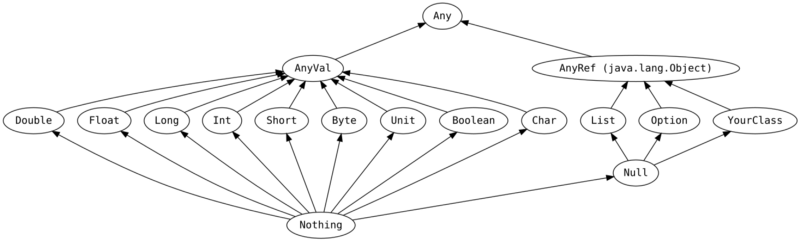
\includegraphics[width=\textwidth]{scalaTypeHierarchy}
\centering
\end{figure}

Every basic Scala type inherits from \texttt{AnyVal}. On the other side, \texttt{AnyRef} is an alias for \texttt{java.lang.Object}. Lastly, both \texttt{AnyVal} and \texttt{AnyRef} inherits from \texttt{Any}.

\subparagraph{Numeric types}:
\begin{lstlisting}[language=scala, style=snippet]
1 + 1   // 2
2 - 1   // 1
5 * 3   // 15
6 / 2   // 3
6 / 4   // 1
6.0 / 4 // 1.5
6 / 4.0 // 1.5
\end{lstlisting}

\subparagraph{Booleans.} Scala supports the Boolean values \texttt{true} an \texttt{false}, as well as the common Boolean operations.
\begin{lstlisting}[language=scala, style=snippet]
!true         // false
!false        // true
true == false // false
10 > 5        // true
\end{lstlisting}

\subparagraph{Strings}
Strings are surrounded by double quotes. Single quotes only used for chars. Triple double-quotes let strings span multiple rows and contain quotes.
\begin{lstlisting}[language=scala, style=snippet]
"Scala strings are surrounded by double quotes"
'a' // A Scala Char
val html = """<form id="daform">
                <p>Press belo', Joe</p>
                <input type="submit">
              </form>"""
\end{lstlisting}
\undline{String interpolation} can be used to embed values directly in string literals.
\begin{lstlisting}[language=scala, style=snippet]
val name = "Bob"
println(s"Hello $name!") // Hello Bob!
\end{lstlisting}
The \texttt{s} before the string is a \udef{string interpolator}. Out of the box Scala provides three string interpolators, but we can create our own as well.
\begin{enumerate}
\item The \textbf{\texttt{s} interpolator} allows variables to be inserted into a string, as shown above. Arbitrary expressions can also be inserted:
\begin{lstlisting}[language=scala, style=snippet]
println(s"1 + 1 = ${1 + 1}")
\end{lstlisting}
\item The \textbf{\texttt{f} interpolator} allows creation of formatted strings. All variable references should be followed by a format string:
\begin{lstlisting}[language=scala, style=snippet]
val height = 1.9d
val name = "James"
println(f"$name%s is $height%2.2f meters tall")  // James is 1.90 meters tall
\end{lstlisting}
Allowed format strings are outlines in the Formatter javadoc: \url{https://docs.oracle.com/javase/6/docs/api/java/util/Formatter.html#detail}
The \texttt{f} interpolator is typesafe. If you try to pass a format string that only works for integers but pass a double, the compiler will issue an error.
\item The \textbf{\texttt{raw} interpolator} is like the \texttt{s} interpolator, except it performs no escaping of literals within the string.
\begin{lstlisting}[language=scala, style=snippet]
scala> raw"a\nb"
res1: String = a\nb
\end{lstlisting}
\end{enumerate}

\subparagraph{Array.} Instantiation using an array literal and accessing elements of an array works as follows (with type inference):
\begin{lstlisting}[language=scala, style=snippet]
val a = Array(1, 2, 3, 5, 8, 13)
a(0)     // Int = 1
a(3)     // Int = 5
a(21)    // Throws an exception
\end{lstlisting}
We can also declare an array as follows
\begin{lstlisting}[language=scala, style=snippet]
val a = new Array[Int](2)
a(0) = 5
a(1) = 2
\end{lstlisting}
Despite being declared as a \texttt{val} in this example, the \texttt{Array} object is mutable so we can change the value of indexes $0$ and $1$. The designation \texttt{val} just means \texttt{a} cannot reference a different array. The array itself may be modified in situ.

A \textbf{\texttt{List}} is like an array, but is immutable.

\subparagraph{Map.} Initialization is as follows:
\begin{lstlisting}[language=scala, style=snippet]
val colours = Map("red" -> "#FF0000", "azure" -> "#F0FFFF", "peru" -> "#CD853F")
colours("red") // java.lang.String = FF0000
\end{lstlisting}
A \texttt{Map} is an immutable data structure. Adding an element means creating another \texttt{Map}.

Maps can have a default value:
\begin{lstlisting}[language=scala, style=snippet]
val safeColours = safeColours.withDefaultValue("Unknown")
safeColours("green")   // java.lang.String = "Unknown"
\end{lstlisting}

Mutable maps exist in \texttt{scala.collection.mutable.Map}.
\begin{lstlisting}[language=scala, style=snippet]
val states = scala.collection.mutable.Map("AL" -> "Alabama", "AK" -> "tobedefined")
states("AK") = "Alaska"
\end{lstlisting}

\subparagraph{Sets} are Iterables that contain no duplicate elements. We test for set membership with parentheses.
\begin{lstlisting}[language=scala, style=snippet]
val s = Set(1, 3, 7)
s(0)      // Boolean = false
s(1)      // Boolean = true
\end{lstlisting}

\subparagraph{Tuples} are immutable and contain a fixed number of elements, each with a distinct type. Literals use parentheses.
\begin{lstlisting}[language=scala, style=snippet]
val d = (3, 1, "five")
(colours, states)
\end{lstlisting}
Accessing elements of tuples is done with \texttt{.\_n}, where \texttt{n} is the 1-based index of the element.
\begin{lstlisting}[language=scala, style=snippet]
d._1    // Int = 3
d._2    // Int = 1
\end{lstlisting}
Tuples can also be unpacked:
\begin{lstlisting}[language=scala, style=snippet]
val (div, mod) = divideInts(10, 3)
div     // Int = 3
mod     // Int = 1
\end{lstlisting}

\paragraph{Flow control}
\begin{itemize}
\item \textbf{If-else}
\begin{lstlisting}[language=scala, style=snippet]
if (condition1) {

} else if (condition2) {

} else {

}
\end{lstlisting}
It is also an expression.
\begin{lstlisting}[language=scala, style=snippet]
def max(x: Int, y: Int) = if (x > y) x else y
\end{lstlisting}
\item Basic for loop:
\begin{lstlisting}[language=scala, style=snippet]
// a goes from 0 to 10 inclusive
for (a <- 0 to 10) {
  println(a)
}
// a goes from 0 to 10 exclusive
for (a <- 0 until 10) {
  println(a)
}
// Looping over two elements
for (a <- 0 until 2; b <- 0 to 2) {
  println((a,b))
}
\end{lstlisting}
\item Looping over iterable (with optional condition):
\begin{lstlisting}[language=scala, style=snippet]
for (elem <- list if elem % 2 == 0) {
  
}
\end{lstlisting}
\item For comprehension functions as a generator
\begin{lstlisting}[language=scala, style=snippet]
val sub = for (elem <- list if elem % 2 == 0) yield elem
\end{lstlisting}
\end{itemize}
Exceptions can be handled in two ways.
\begin{lstlisting}[language=scala, style=snippet]
try {
  val n = new FileReader("input.txt").read()
  println(s"Success: $n")
} catch {
  case e: Exception =>
    e.printStackTrace
}
\end{lstlisting}
Or using \texttt{Try}.
\begin{lstlisting}[language=scala, style=snippet]
val tried: Try[Int] = Try(new FileReader("notes.md")).map(f => f.read())
    
tried match {
  case Success(n) => println(s"Success: $n")
  case Failure(e) => e.printStackTrace
}
\end{lstlisting}

\paragraph{Methods.}
A method is a function that is a member of a class, trait or object.
A basic method example:
\begin{lstlisting}[language=scala, style=snippet]
def add(x: Int, y: Int): Int = {
  x + y
}
\end{lstlisting}
Parameters are immutable. The \texttt{return} keyword is optional. The method will automatically return the last expression. \texttt{return} exits the current method, not the current block (as opposed to Java).
 
The return type is optional. The Scala compiler is also able to infer it.

Methods without output can be written two ways
\begin{lstlisting}[language=scala, style=snippet]
def printSomething(s: String) = {
  println(s)
}
def printSomething(s: String): Unit = {
  println(s)
}
\end{lstlisting}
Multiple outputs can be returned using tuples.
\begin{lstlisting}[language=scala, style=snippet]
def increment(x: Int, y: Int): (Int, Int) = {
  (x + 1, y + 1)
}
\end{lstlisting}
A method without arguments can be called without parentheses. Best practice dictates that this syntax is to be used if the method does not have any side-effects. (See also the \texttt{Dog} class below).

The last parameter can be allowed to take any number of arguments, using an asterisk
\begin{lstlisting}[language=scala, style=snippet]
def variablesArguments(args: Int*): Int = {
  var n = 0
  for (arg <- args) {
    n += arg
  }
  n
}
\end{lstlisting}
We can also give parameters default values. The default parameter may be used by providing \texttt{\_} as an argument (or using named arguments).
\begin{lstlisting}[language=scala, style=snippet]
def default(x: Int = 1, y: Int): Int = {
  x * y
}
default(_, 3)  // Int = 3
default(y = 3) // Int = 3
\end{lstlisting}

Methods may also be nested inside other methods.

\paragraph{Functions.}
Functions are first-class in Scala. This means methods can take a function as a parameter.
\begin{lstlisting}[language=scala, style=snippet]
def foo(i: Int, f: Int => Int): Int = {
  f(i)
}
\end{lstlisting}
Function literals defined as follows
\begin{lstlisting}[language=scala, style=snippet]
val increment: Int => Int = (x: Int) => x + 1
val divideInts: (Int, Int) => (Int, Int) = (x: Int, y: Int) => (x / y, x % y)
\\ Or, using type inference:
val divideInts = (x: Int, y: Int) => (x / y, x % y)
\end{lstlisting}
By not assigning a function to a variable, we get an anonymous function.

Scala supports closures.

Partial functions can be implemented with the following syntax
\begin{lstlisting}[language=scala, style=snippet]
def speed(distance: Float, time: Float): Float = {
  distance / time
}
val partialSpeed: Float => Float = speed(5, _)
\end{lstlisting}

\paragraph{Classes, objects and traits}
\subparagraph{Classes} Example of a class:
\begin{lstlisting}[language=scala, style=snippet]
class Dog(br: String) {
  var breed: String = br
  def bark = "Woof, woof!"

  private def sleep(hours: Int) =
    println(s"I'm sleeping for $hours hours")
}

val mydog = new Dog("greyhound")
println(mydog.breed) // => "greyhound"
println(mydog.bark) // => "Woof, woof!"
\end{lstlisting}
Values and methods are assumed public. Values declared with \texttt{val} cannot be changed. \texttt{protected} (members are only accessible from sub-classes) and \texttt{private} (members are only accessible from the current class/object) keywords are also available. We can also make a method private only outside a package.

Scala supports two types of constructors:
\begin{enumerate}
\item The \textbf{primary constructor} is anything defined in the body of the class except method declarations. The parameter list comes after the class name and may contain default values. It may be omitted. Only a primary constructor is allowed to invoke a superclass constructor. A primary constructor may be made private by using the \texttt{private} keyword between the class name and the constructor parameter-list.
\item \textbf{Auxiliary contructors} are like methods with the name \texttt{this}. They must call a previously defined constructor, i.e. a primary or auxiliary constructor that lexically precedes it. The first statement of the auxiliary constructor must contain the constructor call using \texttt{this}.
\begin{lstlisting}[language=scala, style=snippet]
class GFG( Aname: String, Cname: String) 
{ 
    var no: Int = 0;; 
    def display() 
    { 
        println("Author name: " + Aname); 
        println("Chapter name: " + Cname); 
        println("Total number of articles: " + no); 
          
    } 
      
    // Auxiliary Constructor 
    def this(Aname: String, Cname: String, no:Int)  
    { 
        // Invoking primary constructor 
        this(Aname, Cname) 
        this.no=no 
    } 
} 
\end{lstlisting}
\end{enumerate}

Abstract methods are methods with no body. A class with abstract methods must be declared \texttt{abstract}.
\begin{lstlisting}[language=scala, style=snippet]
abstract class Dog(br: String) {
  var breed: String = br
  def chaseAfter(what: String): String
}
\end{lstlisting}

\subparagraph{Objects} The \texttt{object} keyword creates a type and a singleton instance of it. Objects and classes can have the same name.
\begin{lstlisting}[language=scala, style=snippet]
object Dog {
  def allKnownBreeds = List("pitbull", "shepherd", "retriever")
  def createDog(breed: String) = new Dog(breed)
}
\end{lstlisting}

\subparagraph{Case classes} Case classes are like classes, but are primarily used to create data containers. They are immutable. Classes proper tend to focus on objects oriented concept, such as encapsulation, polymorphism, and behavior. The values tend to be private and only the methods exposed.

\begin{lstlisting}[language=scala, style=snippet]
case class Person(name: String, phoneNumber: String)

val george = Person("George", "1234")
val kate = Person("Kate", "4567")
\end{lstlisting}
Cases classes don't need \texttt{new}.

Case classes have extra functionality built in, such as
\begin{itemize}
\item getters
\begin{lstlisting}[language=scala, style=snippet]
george.phoneNumber  // => "1234"
\end{lstlisting}
\item per field equality (no need to override .equals)
\begin{lstlisting}[language=scala, style=snippet]
Person("George", "1234") == Person("Kate", "1236")  // => false
\end{lstlisting}
\item easy way to copy
\begin{lstlisting}[language=scala, style=snippet]
val otherGeorge = george.copy(phoneNumber = "9876")
\end{lstlisting}
\end{itemize}

\subparagraph{Traits}
Similar to Java interfaces, traits define an object type and method signatures. Scala allows partial implementation of those methods. Constructor parameters are not allowed. Traits can inherit from other traits or classes without parameters. A trait method can also have a default implementation.
\begin{lstlisting}[language=scala, style=snippet]
trait Dog {
    def breed: String
    def color: String
    def bark: Boolean = true
    def bite: Boolean
}
class SaintBernard extends Dog {
    val breed = "Saint Bernard"
    val color = "brown"
    def bite = false
}
\end{lstlisting}
A trait can also be used as a mixin. The class ``extends'' the first trait, but the keyword \texttt{with} can add additional traits.
\begin{lstlisting}[language=scala, style=snippet]
trait Bark {
    def bark: String = "Woof"
}
trait Dog {
    def breed: String
    def color: String
}
class SaintBernard extends Dog with Bark {
    val breed = "Saint Bernard"
    val color = "brown"
}
\end{lstlisting}

\paragraph{Generics}
TODO

\paragraph{Pattern matching}
Like a switch statement, but much more powerful.
\begin{lstlisting}[language=scala, style=snippet]
def matchEverything(obj: Any): String = obj match {
  // You can match values:
  case "Hello world" => "Got the string Hello world"

  // You can match by type:
  case x: Double => "Got a Double: " + x

  // You can specify conditions:
  case x: Int if x > 10000 => "Got a pretty big number!"

  // You can match case classes as before:
  case Person(name, number) => s"Got contact info for $name!"

  // You can match regular expressions:
  case email(name, domain) => s"Got email address $name@$domain"

  // You can match tuples:
  case (a: Int, b: Double, c: String) => s"Got a tuple: $a, $b, $c"

  // You can match data structures:
  case List(1, b, c) => s"Got a list with three elements and starts with 1: 1, $b, $c"

  // You can nest patterns:
  case List(List((1, 2, "YAY"))) => "Got a list of list of tuple"

  // Match any case (default) if all previous haven't matched
  case _ => "Got unknown object"
}
\end{lstlisting}

\paragraph{Currying and implicits} TODO

\paragraph{Concurrency}
TODO
\subsection{Eiffel}
Design by contract.

\section{Interpreted languages}
These are general-purpose programming languages that typically support multiple paradigms.
\subsection{Python}
special * syntax

 PEP 3107 -- Function Annotations
 PEP 484 -- Type Hints
\subsubsection{Implementations}
CPython, PyPy.
\subsection{Javascript}
\subsection{Lua}
\subsection{Perl}
\subsection{R}
\paragraph{History, purpose and setup}

\paragraph{Syntax}
\begin{itemize}
\item In the interpreter you can get help about \textit{word} using \texttt{?\textit{word}}.
\item \textbf{Comments}
\begin{lstlisting}[language={r}, style=snippet]
# Single line comments begin with a '#'
# There are no multiline comments.
\end{lstlisting}
item \textbf{Variables} can be assigned in different ways:
\begin{lstlisting}[language={r}, style=snippet]
x = 5     # this is possible
y <- "1"  # this is preferred
TRUE -> z # this works but is weird
\end{lstlisting}
\end{itemize}

\paragraph{Data and datatypes}
You can find out the type of any expression using \texttt{class()}:
\begin{lstlisting}[language={r}, style=snippet]
class(5) # "numeric"
\end{lstlisting}

\subparagraph{Basic types}:
\begin{itemize}
\item \textbf{Numeric} is a double-precision floating-point number.
\begin{lstlisting}[language={r}, style=snippet]
# Unless otherwise specified all numbers are assumed to be numerics
class(5)    # "numeric"
class(12.2) # "numeric"
# You can have infinitely large or small numbers
class(Inf)  # "numeric"
class(-Inf) # "numeric"
# You can also use scientific notation
5e4 # 50000
6.02e23 # Avogadro's number
1.6e-35 # Planck length
\end{lstlisting}
Illegal arithmetic yields a value \texttt{NaN} (``not-a-number''):
\begin{lstlisting}[language={r}, style=snippet]
0 / 0 # NaN
class(NaN) # "numeric"
\end{lstlisting}
\item\textbf{Integers} Long-storage integers are written with L.
\begin{lstlisting}[language={r}, style=snippet]
5L # 5
class(5L) # "integer"
\end{lstlisting}
\item \textbf{Character} There is no difference between strings and characters in R. To write a string literal both single and double quotes can be used.
\begin{lstlisting}[language={r}, style=snippet]
class("Horatio")  # "character"
class('Horatio')  # "character"
class('H')        # "character"
\end{lstlisting}
\item \textbf{Logical} Booleans are logical. Missing data (\texttt{NA}) is as well.
\begin{lstlisting}[language={r}, style=snippet]
class(TRUE)     # "logical"
class(FALSE)    # "logical"
class(NA)       # "logical"
\end{lstlisting}
\item \textbf{Factor} The factor class is for categorical data. Factors can be ordered (like childrens' grade levels) or unordered (like gender).
\item \textbf{NULL} is NULL. It can be used to blank out a vector.
\end{itemize}

\subparagraph{Data structures}
\begin{itemize}
\item \textbf{Vectors} are created with the function \texttt{c()}.
\begin{lstlisting}[language={r}, style=snippet]
c(1, 2, 3, 4)   # 1 2 3 4
vec <- c(8, 9, 10, 11)
vec             # 8 9 10 11
\end{lstlisting}
Every value is considered a vector of length 1. Conversely every vector has the datatype of its contents.
\begin{lstlisting}[language={r}, style=snippet]
class(c(4L, 5L, 8L, 3L)) # "integer"
\end{lstlisting}
A vector can not contain data of different types, but it may always contain the logical value \texttt{NA}.

R indexes from $1$. Slicing is also supported (bounds are inclusive).
\begin{lstlisting}[language={r}, style=snippet]
vec[1]    # 8
vec[2:3]  # 9 10
\end{lstlisting}

Some other ways of creating vectors include
\begin{lstlisting}[language={r}, style=snippet]
5:15                      # 5  6  7  8  9 10 11 12 13 14 15
seq(from=0, to=11, by=2)  # 0  2  4  6  8 10
\end{lstlisting}
\item \textbf{Matrices} are two-dimensional vectors. All entries are of the same type. Unlike a vector, the class of a matrix is ``matrix'', no matter what's in it.
\begin{lstlisting}[language={r}, style=snippet]
mat <- matrix(nrow = 4, ncol = 3, c(1,2,3,4,5,6))
mat
# =>
#       [,1] [,2] [,3]
# [1,]    1    5    3
# [2,]    2    6    4
# [3,]    3    1    5
# [4,]    4    2    6

class(mat) # "matrix"
\end{lstlisting}
Indexing for matrices:
\begin{lstlisting}[language={r}, style=snippet]
# Ask for vector containing the first row
mat[1,]    # 1 5 3
# Ask for a specific cell
mat[3,2]   # 1
\end{lstlisting}
Matrices can be made by sticking vectors together, either as rows or as columns.
\begin{lstlisting}[language={r}, style=snippet]
rbind(c(1,2,4,5), c(6,7,0,4))
# =>
#      [,1] [,2] [,3] [,4]
# [1,]    1    2    4    5
# [2,]    6    7    0    4
cbind(1:4, c("dog", "cat", "bird", "dog"))
# =>
#      [,1] [,2]
# [1,] "1"  "dog"
# [2,] "2"  "cat"
# [3,] "3"  "bird"
# [4,] "4"  "dog"
\end{lstlisting}
\item \textbf{Data frames} are two-dimensional structures that can contain different types. The class of a data frame is ``data.frame''.
\begin{lstlisting}[language={r}, style=snippet]
students <- data.frame(c("Cedric","Fred","George","Cho","Draco","Ginny"),
                       c(3,2,2,1,0,-1),
                       c("H", "G", "G", "R", "S", "G"))
names(students) <- c("name", "year", "house") # name the columns
class(students)   # "data.frame"
students
# =>
#     name year house
# 1 Cedric    3     H
# 2   Fred    2     G
# 3 George    2     G
# 4    Cho    1     R
# 5  Draco    0     S
# 6  Ginny   -1     G
\end{lstlisting}
The \texttt{data.frame()} function converts character vectors to factor vectors by default; turn this off by setting \texttt{stringsAsFactors = FALSE} when you create the data frame.

Indexing data frames:
\begin{lstlisting}[language={r}, style=snippet]
students$year      # 3  2  2  1  0 -1
students[,2]       # 3  2  2  1  0 -1
students[,"year"]  # 3  2  2  1  0 -1
\end{lstlisting}
A column can be dropped by assigning the \texttt{NULL} value to it.
\begin{lstlisting}[language={r}, style=snippet]
students$house <- NULL
students
# =>
#     name year
# 1 Cedric    3
# 2   Fred    2
# 3 George    2
# 4    Cho    1
# 5  Draco    0
# 6  Ginny   -1
\end{lstlisting}
Rows can be dropped by subsetting:
\begin{lstlisting}[language={r}, style=snippet]
students[students$house != "G",]
# =>
#     name year house
# 1 Cedric    3     H
# 4    Cho    1     R
# 5  Draco    0     S
\end{lstlisting}
\item \textbf{Arrays} are $n$-dimensional structures that contain only one type.
\begin{lstlisting}[language={r}, style=snippet]
array(c(c(c(2,300,4),c(8,9,0)),c(c(5,60,0),c(66,7,847))), dim=c(3,2,2))
# =>
# , , 1
#
#      [,1] [,2]
# [1,]    2    8
# [2,]  300    9
# [3,]    4    0
#
# , , 2
#
#      [,1] [,2]
# [1,]    5   66
# [2,]   60    7
# [3,]    0  847
\end{lstlisting}
\item \textbf{Lists} are like dictionaries in Python. May be multi-dimensional. Possibly ragged. May contain different types.
\begin{lstlisting}[language={r}, style=snippet]
list1 <- list(time = 1:40)
list1$price = c(rnorm(40,.5*list1$time,4))
\end{lstlisting}
List indexing can be done in several ways. The following are equivalent in this case:
\begin{lstlisting}[language={r}, style=snippet]
list1$time
list1[["time"]]
list1[[1]]
\end{lstlisting}
Lists are not very efficient.
\end{itemize}

\subparagraph{Type coercion}
\begin{lstlisting}[language={r}, style=snippet]
as.character(c(6, 8)) # "6" "8"
as.logical(c(1,0,1,1)) # TRUE FALSE  TRUE  TRUE
as.numeric("Bilbo")
# =>
# [1] NA
# Warning message:
# NAs introduced by coercion
\end{lstlisting}
If you put elements of different types into a vector, weird coercions happen:
\begin{lstlisting}[language={r}, style=snippet]
c(TRUE, 4) # 1 4
c("dog", TRUE, 4) # "dog"  "TRUE" "4"
\end{lstlisting}

\paragraph{Basic operations and arithmetic}
\subparagraph{Comparisons}
\begin{lstlisting}[language={r}, style=snippet]
TRUE == FALSE   # FALSE
FALSE != TRUE   # TRUE
\end{lstlisting}
\subparagraph{Numbers} Doing arithmetic on a mix of integers and numerics returns a numeric. Arithmetic on integers returns integers (except with division).
\begin{lstlisting}[language={r}, style=snippet]
10L + 66L # 76
53.2 - 4  # 49.2
2.0 * 2L  # 4
3L / 4    # 0.75    # dividing always returns numeric
4 ^ 2     # 16
4 %% 3.1  # 0.9     # modulo
4 %% 3.1  # 0.9     # modulo
\end{lstlisting}
\subparagraph{Logicals}
\begin{lstlisting}[language={r}, style=snippet]
# OR
TRUE | FALSE    # TRUE
TRUE | NA       # TRUE
FALSE | NA      # NA
NA | NA         # NA

# AND
TRUE & FALSE    # FALSE
TRUE & NA       # NA
FALSE & NA      # FALSE
NA & NA         # NA
\end{lstlisting}
\subparagraph{Vectors}
\begin{itemize}
\item Arithmetic with vectors of the same length pairs up the elements
\begin{lstlisting}[language={r}, style=snippet]
c(1,2,3) + c(1,2,3) # 2 4 6
\end{lstlisting}
\item Arithmetic with scalars is applied element-wise to the vector
\begin{lstlisting}[language={r}, style=snippet]
(4 * c(1,2,3) - 2)  # 2 6 10
\end{lstlisting}
\item Arithmetic with vectors of different length can only be done if the length of the larger vector is an integer multiple of the length of the smaller. The smaller vector is then repeated enough times to fill the larger. This is a generalisation of the above two behaviours. Usually it is better practice and easier to read if lengths are matched.
\begin{lstlisting}[language={r}, style=snippet]
c(1,2,3,1,2,3) * c(1,2)          # 1 4 3 2 2 6
c(1,2,3,1,2,3) * c(1,2,1,2,1,2)  # 1 4 3 2 2 6

c('Z', 'o', 'r', 'r', 'o') == "Zorro"  # FALSE FALSE FALSE FALSE FALSE
c('Z', 'o', 'r', 'r', 'o') == "Z"      # TRUE FALSE FALSE FALSE FALSE
# (Remember every value is treated as a vector of length 1)
\end{lstlisting}
\end{itemize}
\subparagraph{Matrices}
Matrices can be transposed and multiplied.
\begin{lstlisting}[language={r}, style=snippet]
mat
# =>
#      [,1] [,2]
# [1,]    1    4
# [2,]    2    5
# [3,]    3    6
t(mat)
# =>
#      [,1] [,2] [,3]
# [1,]    1    2    3
# [2,]    4    5    6
mat %*% t(mat)
# =>
#      [,1] [,2] [,3]
# [1,]   17   22   27
# [2,]   22   29   36
# [3,]   27   36   45
\end{lstlisting}

\paragraph{Flow control and loops}
\begin{itemize}
\item \textbf{If/else}
\begin{lstlisting}[language={r}, style=snippet]
if (4 > 3) {
    print("4 is greater than 3")
} else {
    print("4 is not greater than 3")
}
\end{lstlisting}
\item \textbf{For loops}
\begin{lstlisting}[language={r}, style=snippet]
for (i in 1:4) {
  print(i)
}
\end{lstlisting}
\item \textbf{While loops}
\begin{lstlisting}[language={r}, style=snippet]
a <- 10
while (a > 4) {
    cat(a, "...", sep = "")
    a <- a - 1
})
\end{lstlisting}
\end{itemize}
Loops run slowly in R. It is generally much better to do operations on entire vectors or use \texttt{apply()}-type functions.

\paragraph{Environments}

\paragraph{Functions}

\begin{lstlisting}[language={r}, style=snippet]
jiggle <- function(x) {
    x = x + rnorm(1, sd=.1) #add in a bit of (controlled) noise
    return(x)
}
# Called like any other R function:
jiggle(5)
\end{lstlisting}

\paragraph{Built-in functionality}
\begin{itemize}
\item \textbf{Constants}
\begin{enumerate}
\item[\texttt{letters}]
\item[\texttt{month.abb}]
\end{enumerate}
\item \textbf{Numeric functions}
\begin{enumerate}
\item[\texttt{round()}]
\item[\texttt{log()}]
\item[\texttt{max()}]
\end{enumerate}
\item \textbf{Logical functions}
\begin{enumerate}
\item[\texttt{isTRUE()}]
\end{enumerate}
\item \textbf{Functions on strings}
\begin{enumerate}
\item[\texttt{substr()}]
\item[\texttt{gsub()}]
\end{enumerate}
\item \textbf{Functions on vectors}
\begin{enumerate}
\item[\texttt{length()}]
\item[\texttt{sort()}]
\item[\texttt{which()}] Return indices of elements that match.
\item[\texttt{any()}] Return true if any of the elements match.
\item[\texttt{max()}]
\item[\texttt{min()}]
\item[\texttt{sum()}]
\item[\texttt{head()}] Look at top of dataset.
\item[\texttt{tail()}] Look at bottom of dataset.
\end{enumerate}
\textbf{Descriptive statistics}
\begin{enumerate}
\item[\texttt{data()}] Browse pre-loaded data sets
\item[\texttt{data(rivers)}] Load dataset ``Lengths of Major North American Rivers'' as a numeric vector \texttt{rivers}.
\item[\texttt{mean()}]
\item[\texttt{var()}]
\item[\texttt{sd()}]
\item[\texttt{summary(rivers)}] Summary statistics: minimum, 1st quartile, median, mean, 3rd quartile, maximum.
\end{enumerate}
\item \textbf{Functions on data frames}
\begin{enumerate}
\item[\texttt{dim()}]
\item[\texttt{nrow()}]
\item[\texttt{ncol()}]
\end{enumerate}
\item \textbf{Data visualisation}
\begin{itemize}
\item[\textbf{Stem-and-leaf}]
\item[\textbf{Histogram}]
\item[\textbf{Plot}]
\end{itemize}
\end{itemize}

\paragraph{Packages}
The \texttt{data.table} package provides functionality a lot like the data frames.
\begin{lstlisting}[language={r}, style=snippet]
# An augmented version of the data.frame structure is the data.table
# If you're working with huge or panel data, or need to merge a few data
# sets, data.table can be a good choice. Here's a whirlwind tour:
install.packages("data.table") # download the package from CRAN
require(data.table) # load it
students <- as.data.table(students)
students # note the slightly different print-out
# =>
#      name year house
# 1: Cedric    3     H
# 2:   Fred    2     G
# 3: George    2     G
# 4:    Cho    1     R
# 5:  Draco    0     S
# 6:  Ginny   -1     G
students[name=="Ginny"] # get rows with name == "Ginny"
# =>
#     name year house
# 1: Ginny   -1     G
students[year==2] # get rows with year == 2
# =>
#      name year house
# 1:   Fred    2     G
# 2: George    2     G
# data.table makes merging two data sets easy
# let's make another data.table to merge with students
founders <- data.table(house=c("G","H","R","S"),
                       founder=c("Godric","Helga","Rowena","Salazar"))
founders
# =>
#    house founder
# 1:     G  Godric
# 2:     H   Helga
# 3:     R  Rowena
# 4:     S Salazar
setkey(students, house)
setkey(founders, house)
students <- founders[students] # merge the two data sets by matching "house"
setnames(students, c("house","houseFounderName","studentName","year"))
students[,order(c("name","year","house","houseFounderName")), with=F]
# =>
#    studentName year house houseFounderName
# 1:        Fred    2     G           Godric
# 2:      George    2     G           Godric
# 3:       Ginny   -1     G           Godric
# 4:      Cedric    3     H            Helga
# 5:         Cho    1     R           Rowena
# 6:       Draco    0     S          Salazar

# data.table makes summary tables easy
students[,sum(year),by=house]
# =>
#    house V1
# 1:     G  3
# 2:     H  3
# 3:     R  1
# 4:     S  0
\end{lstlisting}

\section{Functional languages}
\subsection{Functional programming paradigm}
pure state, 
\subsection{LISP}
\subsection{Scheme}
Continuations?
\subsection{ML}
\subsection{Haskell}
\paragraph{History.}

\paragraph{Concepts.}
Haskell has \udef{lazy evaluation}; it only evaluates things when it needs to.

\paragraph{Basic setup.}
Haskell can be run in a REPL (Read-Eval-Print Loop). The REPL can be started with the command \texttt{ghci}.

In the REPL, new values are created with \texttt{let}.
\begin{lstlisting}[language=haskell, style=snippet]
let foo = 5
\end{lstlisting}
Type can be inspected using \texttt{:t}.
\begin{lstlisting}[language=haskell, style=snippet]
> :t foo
foo :: Integer
\end{lstlisting}
Additional information on any identifier is given by \texttt{:i}:
\begin{lstlisting}[language=haskell, style=snippet]
> :i (+)
class Num a where
  (+) :: a -> a -> a
  ...
    -- Defined in 'GHC.Num'
infixl 6 +
\end{lstlisting}


\paragraph{Syntactic elements.}
Comments:
\begin{lstlisting}[language=haskell, style=snippet]
-- Single line comments start with two dashes.
{- Multiline comments can be enclosed
in a block like this.
-}
\end{lstlisting}
Lines end with a newline character.

\paragraph{Primitive data types and operators.}
\subparagraph{Numbers.}
Math is a you expect. Division is floating point by default. Integer division done using \texttt{`div`}.
\begin{lstlisting}[language=haskell, style=snippet]
1 + 1 -- 2
8 - 1 -- 7
10 * 2 -- 20
35 / 4 -- 8.75
35 `div` 4 -- 8
\end{lstlisting}
\subparagraph{Booleans.} The primitives \texttt{True} and \texttt{False} are capitalised. Operations:
\begin{lstlisting}[language=haskell, style=snippet]
not True -- False
not False -- True
1 == 1 -- True
1 /= 1 -- False
1 < 10 -- True
\end{lstlisting}
Here \texttt{not} is actually a function.
\subparagraph{Strings and characters.} Strings are lists of characters.
\begin{lstlisting}[language=haskell, style=snippet]
"This is a string."
'a' -- character
'You cant use single quotes for strings.' -- error!

['H', 'e', 'l', 'l', 'o'] -- "Hello"
"This is a string" !! 0 -- 'T'
\end{lstlisting}

Function identifiers do not need to contain letters.
\begin{lstlisting}[language=haskell, style=snippet]
(//) a b = a `div` b
35 // 4 -- 8
\end{lstlisting}
\paragraph{Lists and tuples.}
\subparagraph{Lists.}
Every element in a list must have the same type. Ranges can be used and are versatile.
\begin{lstlisting}[language=haskell, style=snippet]
[1, 2, 3, 4, 5]
[1..5]              -- [1, 2, 3, 4, 5]
['A'..'F']          -- "ABCDEF"
[0,2..10] -- [0, 2, 4, 6, 8, 10]
[5..1] -- [] (Haskell defaults to incrementing)
[5,4..1] -- [5, 4, 3, 2, 1]
\end{lstlisting}
Indexing is zero-based and done using \texttt{!!}.
\begin{lstlisting}[language=haskell, style=snippet]
[1..10] !! 3 -- 4
\end{lstlisting}
Thanks to lazy evaluation the following is possible:
\begin{lstlisting}[language=haskell, style=snippet]
[1..] -- a list of all the natural numbers
[1..] !! 999 -- 1000
\end{lstlisting}
List operations:
\begin{lstlisting}[language=haskell, style=snippet]
-- joining two lists
[1..5] ++ [6..10]

-- adding to the head of a list
0:[1..5] -- [0, 1, 2, 3, 4, 5]

head [1..5] -- 1
tail [1..5] -- [2, 3, 4, 5]
init [1..5] -- [1, 2, 3, 4]
last [1..5] -- 5
\end{lstlisting}
List comprehension:
\begin{lstlisting}[language=haskell, style=snippet]
[x*2 | x <- [1..5]] -- [2, 4, 6, 8, 10]
[x*2 | x <- [1..5], x*2 > 4] -- [6, 8, 10]
\end{lstlisting}

\subparagraph{Tuples.} Every element in a tuple can be a different type, but a tuple has a fixed length. Tuple literals are written with parentheses.
\begin{lstlisting}[language=haskell, style=snippet]
("haskell", 1)

-- accessing elements of a pair (i.e. a tuple of length 2)
fst ("haskell", 1) -- "haskell"
snd ("haskell", 1) -- 1

-- pair element accessing does not work on n-tuples (i.e. triple, quadruple, etc)
snd ("snd", "can't touch this", "da na na na") -- error! see function below
\end{lstlisting}

\paragraph{Functions.}
Declaring and calling functions.
\begin{lstlisting}[language=haskell, style=snippet]
add a b = a + b
add 1 2 -- 3
\end{lstlisting}
Haskell also supports infix notation.
\begin{lstlisting}[language=haskell, style=snippet]
1 `add` 2 -- 3
\end{lstlisting}

Branching can be achieved with guards.
\begin{lstlisting}[language=haskell, style=snippet]
fib x
  | x < 2 = 1
  | otherwise = fib (x - 1) + fib (x - 2)
\end{lstlisting}

\subparagraph{Overloading.}
\begin{lstlisting}[language=haskell, style=snippet]
fib 1 = 1
fib 2 = 2
fib x = fib (x - 1) + fib (x - 2)
\end{lstlisting}

\subparagraph{Pattern matching.}
\begin{itemize}
\item On tuples:
\begin{lstlisting}[language=haskell, style=snippet]
sndOfTriple (_, y, _) = y
\end{lstlisting}
\item On lists:
\begin{lstlisting}[language=haskell, style=snippet]
myMap func [] = []
-- x is the first element of the list. 
-- xs is the rest of the list. 
myMap func (x:xs) = func x:(myMap func xs)
\end{lstlisting}
\end{itemize}

\subparagraph{Anonymous functions.} Anonymous functions are created with a backslash followed by all the arguments.
\begin{lstlisting}[language=haskell, style=snippet]
myMap (\x -> x + 2) [1..5] -- [3, 4, 5, 6, 7]
\end{lstlisting}

\subparagraph{Partial application.}
\begin{lstlisting}[language=haskell, style=snippet]
add a b = a + b
foo = add 10 -- foo is now a function that takes a number and adds 10 to it
foo 5 -- 15
-- Another way to write the same thing
foo = (10+)
foo 5 -- 15
\end{lstlisting}

\subparagraph{Function composition.} Function composition is achieved with the \texttt{.} operator.
\begin{lstlisting}[language=haskell, style=snippet]
foo = (4*) . (10+)
foo 5 -- 60 because 4*(10+5) = 60
\end{lstlisting}

\subparagraph{Operator precedence.} The \texttt{\$} operator applies a function to a given parameter. It is low priority and is right-associative. The expression on its right is applied as a parameter to the function on its left.


\subparagraph{Built in functions}

Another \texttt{map} example.
\begin{lstlisting}[language=haskell, style=snippet]
map (*2) [1..5] -- [2, 4, 6, 8, 10]
\end{lstlisting}

foldr, foldl

\paragraph{Type signatures and data types.}
Haskell has a very strong type system, and every valid expression has a type.

Some basic types:
\begin{lstlisting}[language=haskell, style=snippet]
5 :: Integer
"hello" :: String
True :: Bool
\end{lstlisting}

When you define a value, it's good practice to write its type above it:
\begin{lstlisting}[language=haskell, style=snippet]
doubleInt :: Integer -> Integer
doubleInt x = x * 2
\end{lstlisting}

Custom types can be defined.
\begin{lstlisting}[language=haskell, style=snippet]
data Color = Red | Blue | Green
\end{lstlisting}
The type is \texttt{Color} and its possible values are \texttt{Red}, \texttt{Blue} and \texttt{Green}.
Data types can have parameters as well.
\begin{lstlisting}[language=haskell, style=snippet]
data Maybe a = Nothing | Just a
-- These are all of type Maybe
Just "hello"    -- of type `Maybe String`
Just 1          -- of type `Maybe Int`
Nothing         -- of type `Maybe a` for any `a`
\end{lstlisting}

\paragraph{Flow control.}
\subparagraph{\texttt{if}-expressions.}
\begin{lstlisting}[language=haskell, style=snippet]
haskell = if 1 == 1 then "awesome" else "awful" -- haskell = "awesome"
\end{lstlisting}
Multiline \texttt{if}. Indentation is important.
\begin{lstlisting}[language=haskell, style=snippet]
haskell = if 1 == 1
            then "awesome"
            else "awful"
\end{lstlisting}
\subparagraph{\texttt{case} expressions.}
\begin{lstlisting}[language=haskell, style=snippet]
case args of
  "help" -> printHelp
  "start" -> startProgram
  _ -> putStrLn "bad args"
\end{lstlisting}
\subparagraph{Recursion.} Haskell does not have any loops, but we can make them using the \texttt{map} function.
\begin{lstlisting}[language=haskell, style=snippet]
for array func = map func array
for [0..5] $ \i -> show i -- Using the for loop.
\end{lstlisting}


\paragraph{Monads.}
TODO

\paragraph{I/O.}
TODO


\section{Logic programming languages}
\subsection{Planner}
Inspired smalltalk and prolog
\subsection{Prolog}
\paragraph{History}
First specified in 1972. SWI-Prolog offers a comprehensive free Prolog environment.
\paragraph{Concepts}
\begin{itemize}
\item A Prolog database consists of known instances of relations, called \udef{facts}.
\item New relations can be constructed from old ones. These are expressed as \udef{rules}.
\item \udef{Queries} are expressions containing one or more variables.
\item \undline{Unification} is used to determine whether a query has a valid substitution consistent with the rules and facts in the database.
\item \udef{Clauses} are sets of statements.
\end{itemize}

\begin{itemize}
\item A subprogram (called a \udef{predicate}) represents a state of the world.
\item A command (called a \udef{goal}) tells Prolog to make that state of the world true, if possible.
\end{itemize}

\paragraph{Basic setup}
Code entered in interactive mode and code in a file is treated differently. Facts and rules should be put in a file.

The interactive prompt is \texttt{?-} and lines end with a period.


\paragraph{Syntactic elements}
Comments:
\begin{lstlisting}[language=prolog, style=snippet]
% This is a comment
\end{lstlisting}
Facts:
\begin{lstlisting}[language=prolog, style=snippet]
magicNumber(7).
magicNumber(9).
magicNumber(42).
\end{lstlisting}
which we can query:
\begin{lstlisting}[language=prolog, style=snippet]
?- magicNumber(7).                   % True
?- magicNumber(8).                   % False
?- magicNumber(9).                   % True
\end{lstlisting}

Multiple operations can be chained using commas.

\paragraph{Unification}
We request unification by passing an undefined variable:
\begin{lstlisting}[language=prolog, style=snippet]
?- magicNumber(Presto).              % Presto = 7 ;
                                     % Presto = 9 ;
                                     % Presto = 42.
\end{lstlisting}
The equals sign represents unification. We have three cases.
\begin{enumerate}
\item If both sides are bound (i.e., defined), Prolog checks equality.
\item If one side is free (i.e., undefined), Prolog tries to assign the variable to match the other side.
\item If both sides are free, the assignment is remembered.
\end{enumerate}
Attempted unification can have three outcomes. It can
\begin{enumerate}
\item Succeed (return True) without changing anything, because an equality-style unification was true;
\item Succeed (return True) and bind one or more variables in the process; or
\item Fail (return False) because an equality-style unification was false (failure can never bind variables).
\end{enumerate}


The equals sign can not do arithmetic (as Prolog cannot solve equations out of the box). The \texttt{is} operator does allow arithmetic, but right side must always be bound.
\begin{lstlisting}[language=prolog, style=snippet]
?- X = 3+2.             % X = 3+2 - unification can't do arithmetic
?- X is 3+2.            % X = 5 - "is" does arithmetic.
?- 5 = X+2.             % This is why = can't do arithmetic -
                        % because Prolog can't solve equations
?- 5 is X+2.            % Error. Unlike =, the right hand side of IS
                        % must always be bound, thus guaranteeing
                        % no attempt to solve an equation.
\end{lstlisting}
We can however reverse addition if we try to unify with the \texttt{plus} predicate.
\begin{lstlisting}[language=prolog, style=snippet]
?- plus(1, 2, 3).                    % True
?- plus(1, 2, X).                    % X = 3 because 1+2 = X.
?- plus(1, X, 3).                    % X = 2 because 1+X = 3.
?- plus(X, 2, 3).                    % X = 1 because X+2 = 3.
?- plus(X, 5, Y).                    % Error - infinite solutions
\end{lstlisting}

TODO: more

\section{Numerical computing}
\subsection{MATLAB}
\subsection{GNU Octave}
\subsection{Maxima}
\subsection{Julia}

\section{Shell scripting}
\subsection{Bash}
\subsection{DOS}

\section{System and circuit design}
\subsection{SPICE}
\subsection{Verilog}
\subsection{Chisel}
\subsection{FIRRTL}
\subsection{LabVIEW and G}

\section{Database querying}
\subsection{SQL}
\section{Data-interchange}
\subsection{XML}
\subsection{JSON}

\addtocontents{toc}{\protect\setcounter{tocdepth}{5}}

\part{Computer systems}
\setcounter{chapter}{0} % Reset chapter counter
\chapter{Process management and coordination}

\chapter{Memory and storage}
bit, byte, word, kilo / kibi

\chapter{UI / UX}

\chapter{Networking}
TCP / IP etc. ATM

Hosting: firebase

\chapter{Computer security}
A chain is only as strong as its weakest link.
\section{Cryptography}
Shamir's Secret Sharing
\subsection{Stenography}

\chapter{Distributed systems}

\chapter{Operating systems}
POSIX
MBR / UEFI
…
Encoding (Unicode / UTF-8)
...
Console: Bourne, C shell, Bourne-Again, Korn shell, Bash, busybox, DOS, Cygwin, MinGW

Also mobile and game console

\part{Advanced algorithms}
\setcounter{chapter}{0} % Reset chapter counter
\chapter{Artificial intelligence}
\chapter{Machine learning}

\chapter{Simulation}
\section{Overview and problem statement}
\subsection{Time and length scales}
\begin{table}
\centering
\begin{tabular}{llll}
\textbf{Complex structure} & \textbf{Length scale} & \textbf{Time scale} & \textbf{Mechanics} \\ \hline
Complex structure & $10^3$m & $10^{6}$s & structural mechanics \\
Simple structure & $10^1$m & $10^3$s & fracture mechanics \\
Component & $10^{-1}$m & $10^0$s & Continuum mechanics \\
Grain microstructure & $10^{-3}$m & $10^{-3}$s & crystal plasticity \\
Dislocation microstructure & $10^{-5}$m & $10^{-6}$s & micro-mechanics \\
Single dislocation & $10^{-7}$m & $10^{-9}$s & dislocation dynamics \\
Atomic & $10^{-9}$m & $10^{-12}$s & molecular dynamics \\
Electron orbitals & $10^{-11}$m & $10^{-15}$s & quantum mechanics
\end{tabular}
\caption{The important unit structure is indicated for each scale, along with approximate length and time scales, as well as the approach used to simulate the material's behaviour.}
\label{tab:timeLength}
\end{table}
Multiscale modeling: continuum, meso, nano, QM

\subsection{Atomic scale}
Trajectories over potential energy hypersurfaces; MD uses thermal energy to move smoothly over surface, MC moves randomly with probability $\exp(-\Delta U / k_BT)$.

Equilibrium properties ore calculated as mean values over $M$ sampled configurations (assuming the configuration space has been sampled according to the correct distribution)
\[ \bar{f} = \frac{1}{M}\sum^M_{\alpha=1}f_\alpha \]
Law of large numbers:
\[ \Expval{f} = \lim_{M\to \infty}\bar{f} \]

\subsection{Thermodynamic quantities}
\begin{itemize}
\item \textbf{Internal energy} Sum of kinetic and potential energy
\[ U = \bar{K} + \bar{V} \qquad \bar{K} = \sum^N_{i=1}\frac{\bar{p}_i^2}{2m_i} \]
\item \textbf{Temperature} calculated using the equipartition theorem
\[ \bar{K} = \frac{3}{2}Nk_B T \qquad \to \qquad T = \frac{2}{3Nk_B}\bar{K} = \frac{2}{(3N_a - N_c)k_B}\bar{K} \]
where $N_a$ is number of atoms and $N_c$ is the total number of independent constraints.
\item \textbf{Pressure} is calculated using the expression obtained from the virial theorem
\[ p = \frac{N}{V}k_B T + \frac{1}{3V}\sum^N_{i=1}\sum^N_{j>i}\bar{\vec{f}_{ij}\cdot \vec{r}_{ij}} \]
\item \textbf{Free energies} and \textbf{entropy} cannot be calculated directly in general because these are properties of the whole ensemble which require counting all of the ensemble states. There are however some tricks to calculate free energy differences.
\end{itemize}

\subsection{Fluctuations}
Trajectory length must be $>$ decay time of ACF

Time separation must be $\ll$ decay time of ACF.

\subsection{Block averaging}

\section{Monte Carlo simulations}
\subsection{Calculating area under a curve}
\subsection{Importance sampling}
\subsection{Boundary conditions}

\subsection{Markov chain Monte Carlo}
A Markov chain is a stochastic model describing a sequence of events where the probability of the next event occurring only depends on the previous event. In other words we have a chain
\[ X_1 \to X_2 \to \ldots \to X_J \to X_{J+1}\to \ldots \]
and the Markov model is completely determined by the transition probabilities $W(X_J \to X_{J'})$.

\subsection{Metropolis algorithm}
A Monte Carlo algorithm can be used to compute (approximations of) ensemble averages of quantities in statistical mechanics. This is done by sampling the ensemble, calculating the quantity for each sample and then averaging the results.

The tricky part is being able to accurately sample the ensemble. The Metropolis algorithm provides a way to do that with Markov chains. Not all Markov chains sample a well-defined, stationary distribution. A sufficient but not necessary condition for the existence of a stationary distribution is detailed balance.

Detailed balance is essentially microscopic reversibility. For every pair of states $J,J'$ the probability of being in state $J$ and transitioning to $J'$ is the same as being in state $J'$ and transitioning to $J$.
\[ W_{J'\leftarrow J}P^\text{eq}_J = W_{J\leftarrow J'}P^\text{eq}_{J'} \]

It is exactly this stationary distribution $P^\text{eq}_J$ that we want to reflect the ensemble. The equality can be rewritten as
\[ \frac{P^\text{eq}_J}{P^\text{eq}_{J'}} = \frac{W_{J\leftarrow J'}}{W_{J'\leftarrow J}} \]

Next a new and interesting way to generate the Markov chain is introduced. Each state is generated from the previous one using a two-step process:
\begin{enumerate}
\item Propose a new state $J'$. The likelihood of a new state $J'$ being proposed is given by $\alpha_{J'\leftarrow J}$.
\item Decide whether to accept or reject the new state. The new state is accepted with probability $W^\text{acc}_{J'\leftarrow J}$.
\end{enumerate}
The transition probabilities are then given by 
\[ W_{J'\leftarrow J} = \alpha_{J'\leftarrow J}W^\text{acc}_{J'\leftarrow J}. \]
Further imposing detailed balance gives
\[ \frac{P^\text{eq}_J}{P^\text{eq}_{J'}} = \frac{W_{J\leftarrow J'}}{W_{J'\leftarrow J}} = \frac{\alpha_{J\leftarrow J'}W^\text{acc}_{J\leftarrow J'}}{\alpha_{J\leftarrow J'}W^\text{acc}_{J'\leftarrow J}} \]

The beauty of the Metropolis algorithm is that if the underlying stochastic matrix $\alpha$ is symmetric ($\alpha_{J\leftarrow J'} = \alpha_{J'\leftarrow J}$), then this further simplifies to
\[ \frac{P^\text{eq}_J}{P^\text{eq}_{J'}} = \frac{W^\text{acc}_{J\leftarrow J'}}{W^\text{acc}_{J'\leftarrow J}} \]

This means we can choose any $\alpha$ we like (so long as it's symmetric) and we can make sure we are sampling the ensemble correctly by using good rules for accepting new moves.

\subsubsection{Sampling the canonical ensemble}
If we are trying to sample the canonical (NVT) ensemble, we need the stationary distribution the be the Boltzmann distribution.
\[ \frac{P^\text{eq}_J}{P^\text{eq}_{J'}} = \exp\left[- \frac{V_{J'}-V_J}{k_BT}\right] \]
This still leaves some choice as to the exact form of $W^\text{acc}_{J'\leftarrow J}$. The Metropolis choice is
\[ W^\text{acc}_{J'\leftarrow J} = \begin{cases}
\exp\left[- \frac{V_{J'}-V_J}{k_BT}\right] & (V_{J'}>V_J) \\
1 & (V_{J'}\leq V_J)
\end{cases} \]
in other words
\[ W^\text{acc}_{J'\leftarrow J} = \min \left[1, \; \exp\left(-(V_{J'}-V_J) / k_BT\right)\right] \]

TODO write out algorithm

\part{Quantum computation}
\chapter{Circuit model}

\chapter{Eigenpath traversal}
\section{Quantum Zeno effect}
\begin{proposition}
Consider a path of states $\ket{\psi(s)}$ where $s\in[0,1]$. Assume that, for fixed $d$ and all $\delta$,
\[ |\braket{\psi(s)}{\psi(s+\delta}|^2 \geq 1-d^2\delta^2. \]
Then 
\end{proposition}

\section{Adiabatic quantum computation}
\section{Evolution through measurement}
\subsection{Phase randomisation}
$\ket{\psi_0} = \ket{E_0(0)} = \sum_i\alpha_i\ket{E_i(s_1)}$
\begin{align*}
\rho(s_1) &= \frac{1}{T}\int_0^T e^{-iH(s_1)t}\ketbra{\psi_0}{\psi_0} e^{iH(s_1)t} \diff{t} \\
&= \sum_{i,j}\alpha_i\alpha_j^* \frac{1}{T}\left(\int_0^T e^{-i(E_i-E_j)t}\diff{t}\right)\ketbra{E_i}{E_j} \\
&= \sum_{i,j}\alpha_i\alpha_j^* \left(\frac{i(e^{-i(E_i-E_j)T}-1)}{T(E_i-E_j)}\right)\ketbra{E_i}{E_j}
\end{align*}

\begin{theorem}[Randomised dephasing]
Let $\ket{\psi(s)}$ be a nondegenerate eigenstate of $H(s)$ and $\{\omega_j\}$ the energy differences to the other eigenstates $\ket{\psi_j(s)}$. Let $T$ be a random variable. Then, for all states $\rho$, we have
\[ \norm{(M_l - e^{-iH(s)T}\rho e^{-iH(s)T}}_\text{tr} \leq \epsilon = \sup_{\omega_j}|\Phi(\omega_j)| \]
\end{theorem}

\chapter{Variational quantum algorithms}

\chapter{Algorithms}
\section{Grover's search algorithm}
Suppose we have a set $\mathcal{N}$ of $N$ items, some of which are marked. WLOG we can take $\mathcal{N}$ to be the set of bit strings of length $\nu$. The marked items form a subset $\mathcal{M}$ of size $M$. Suppose we have an oracle that tells us whether an object is marked or not:
\[ f:\mathcal{N} \to \{0,1\}: x\mapsto \begin{cases}
0 & (x\in \mathcal{M}) \\
1 & (x\notin \mathcal{M})
\end{cases} \]
Now we want to find a marked item. Classically we need to check $\Theta(N/M)$ items on average.

\subsection{Circuit model}
Let $\setbuilder{\ket{n}}{n\in\mathcal{N}}$ be a basis of a Hilbert space $\mathcal{H}_N$ and let $\mathcal{H}_2$ be a qubit space.

\subsubsection{The oracle}
We would like to use the operator
\[ U_f: \mathcal{H}_N\to \mathcal{H}_N: \ket{n}\mapsto (-1)^{f(n)}\ket{n}. \]

This can be constructed from the oracle
\[ O_f: \mathcal{H}_N\otimes \mathcal{H}_2 \to \mathcal{H}_N\otimes \mathcal{H}_2: \ket{n}\otimes \ket{q}\mapsto \ket{n}\otimes\ket{f(n)\oplus q}, \]
where $\oplus$ is addition modulo $2$, by preparing the qubit in the superposition $\frac{1}{\sqrt{2}}(\ket{0}-\ket{1})$. Then
\begin{align*}
O_f\left(\ket{n}\otimes \frac{1}{\sqrt{2}}(\ket{0}-\ket{1})\right)
&= \ket{n}\otimes \frac{1}{\sqrt{2}}(\ket{f(n)}-\ket{f(n)\oplus 1}) \\
&= (-1)^{f(n)}\ket{n}\otimes \frac{1}{\sqrt{2}}(\ket{0}-\ket{1}).
\end{align*}

The operator $U_f$ can also be written
\[ U_f = \id_{\mathcal{H}_N} - 2\sum_{m\in\mathcal{M}}\ketbra{m}{m}. \]

\subsubsection{The algorithm}
We construct the an initial state which is a superposition of all possible solutions
\[ \ket{\mathcal{N}} = \frac{1}{\sqrt{N}}\sum_{n\in\mathcal{N}}\ket{n}. \]
This can be prepared by applying a Hadamard gate $W$ to each qubit in the register.

We also define the state
\[ \ket{\mathcal{M}} = \frac{1}{\sqrt{M}}\sum_{m\in\mathcal{M}}\ket{m}. \]

We define the operation
\[ U_0 = W^{\otimes\nu}(\id - 2\ketbra{0}{0})W^{\otimes\nu}= \id - 2\ketbra{\mathcal{N}}{\mathcal{N}}. \]

Now both $U_0$ and $U_f$ leave $\Span\{\}$

\subsection{Analogue Grover}
Why does analogue Grover work?


\subsection{Adiabatic Grover}
\[ H_0 = \vec{1} - \ketbra{\mathcal{N}}{\mathcal{N}} = \mathbb{1}-\mathbb{J}/N \]
\[ H_f = \vec{1} - \sum_{m\in\mathcal{M}}\ketbra{m}{m} = \begin{pmatrix}
0 & 0 \\ 0 & \mathbb{1}_{N-M}
\end{pmatrix}.\]

Then
\[ H(s) = (1-s)H_0 + sH_f = \begin{pmatrix}
(1-s)\mathbb{1} +\frac{s-1}{N}\mathbb{J} & \frac{s-1}{N}\mathbb{J} \\
\frac{s-1}{N}\mathbb{J} & \mathbb{1} + \frac{s-1}{N}\mathbb{J}
\end{pmatrix} = \begin{pmatrix}
(1-s)\mathbb{1}_M & 0 \\ 0 & \mathbb{1}_{N-M}
\end{pmatrix} + \frac{s-1}{N}\mathbb{J}. \]
Then, setting $A = \begin{pmatrix}
(1-s-\lambda)\mathbb{1}_M & 0 \\ 0 & (1-\lambda)\mathbb{1}_{N-M}
\end{pmatrix}$
\begin{align*}
\det(H(s)-\lambda) &= \det \left(A + \frac{s-1}{N}\mathbb{J}^{n\times 1}\mathbb{J}^{1\times n}\right) \\
&= \det(A)\det \left(\mathbb{1}_N + \frac{s-1}{N}A^{-1}\mathbb{J}^{n\times 1}\mathbb{J}^{1\times n}\right) \\
&= \det(A)\det \left(1 + \frac{s-1}{N}\mathbb{J}^{1\times n}A^{-1}\mathbb{J}^{n\times 1}\right) \\
&= (1-s-\lambda)^{M}(1-\lambda)^{N-M}\left(1 + \frac{M(s-1)}{(1-s-\lambda)N} + \frac{(N-M)(s-1)}{(1-\lambda)N}\right) \\
&= (1-s-\lambda)^{M-1}(1-\lambda)^{N-M-1}\left(\lambda^2 - \lambda + s(1-s)\frac{N-M}{N}\right),
\end{align*}
where we have used the matrix determinant lemma to simplify the calculation.

We see that there are four distinct eigenvalues:
\begin{align*}
\lambda_{0,1} &= \frac{1}{2}\left(1\pm \frac{\sqrt{N+4(Ns^2-Ns-Ms^2+Ms)}}{\sqrt{N}}\right) &\text{with multiplicity $1$}\\
\lambda_{2} &= 1-s &\text{with multiplicity $M-1$}\\
\lambda_{3} &= 1 &\text{with multiplicity $N-M-1$.}
\end{align*}

Next we are interested in the eigen vectors associated to $\lambda_{0,1}$. Let $Q_1$ be a unitary transformation that maps $\mathbb{J}^{M\times 1}$ to $\begin{pmatrix}
\sqrt{M} \\ 0 \\ 0 \\ \vdots
\end{pmatrix} \in \C^M$. Similarly let $Q_2$ be a unitary transformation that maps $\mathbb{J}^{(N-M)\times 1}$ to $\begin{pmatrix}
\sqrt{N-M} \\ 0 \\ 0 \\ \vdots
\end{pmatrix} \in \C^{(N-M)}$ and define $Q = \begin{pmatrix}
Q_1 & 0 \\ 0 & Q_2
\end{pmatrix}$, which is also unitary. Then we have
\begin{align*}
    QH(s)Q^{-1} &= \begin{pmatrix}
        (1-s)\mathbb{1}_M & 0 \\ 0 & \mathbb{1}_{N-M}
        \end{pmatrix} + \frac{s-1}{N}Q\mathbb{J}^{N\times 1}(\mathbb{J}^{N\times 1})^*Q^* \\
    &= \begin{pmatrix}
        (1-s)\mathbb{1}_M & 0 \\ 0 & \mathbb{1}_{N-M}
        \end{pmatrix} + \frac{s-1}{N} \begin{pmatrix}\sqrt{M} \\ 0 \\ \vdots \\ 0 \\ \sqrt{N-M} \\ 0 \\ \vdots \end{pmatrix}\begin{pmatrix}\sqrt{M} \\ 0 \\ \vdots \\ 0 \\ \sqrt{N-M} \\ 0 \\ \vdots \end{pmatrix}^*.
\end{align*}

All but two of the eigenvectors are just elements of $\mathcal{N}$. To study the other two we can simplify by ``removing the zeros''. Now the eigenvalue problem becomes
\[ \left(\begin{pmatrix}
1-s-\lambda_{0,1} & 0 \\ 0 & 1 -\lambda_{0,1}
\end{pmatrix} + \frac{s-1}{N}\begin{pmatrix}
\sqrt{M} \\ \sqrt{N-M}
\end{pmatrix}\begin{pmatrix}
\sqrt{M} \\ \sqrt{N-M}
\end{pmatrix}^*\right)\vec{v} = 0. \]
Setting $\vec{v} = \begin{pmatrix}
x_1 \\ x_2
\end{pmatrix}$ gives us the equations
\begin{align*}
0 &= (1-s-\lambda_{0,1})x_1 + \frac{s-1}{N}(Mx_1 + \sqrt{M}\sqrt{N-M}x_2)
0 &= (1-\lambda_{0,1})x_2 + \frac{s-1}{N}(\sqrt{M}\sqrt{N-M}x_1 + (N-M)x_2)
\end{align*}
reshuffling and dividing these equations gives
\[ \frac{(1-s-\lambda_{0,1})x_1}{(1-s-\lambda_{0,1})x_2} = \frac{-\frac{s-1}{N}(Mx_1 + \sqrt{M}\sqrt{N-M}x_2)}{-\frac{s-1}{N}(\sqrt{M}\sqrt{N-M}x_1 + (N-M)x_2)} = \frac{\sqrt{M}(\sqrt{M}x_1 + \sqrt{M}\sqrt{N-M}x_2)}{\sqrt{N-M}(\sqrt{M}x_1 + \sqrt{N-M}x_2)} = \frac{\sqrt{M}}{\sqrt{N-M}}. \]
So we have eigenvectors $\vec{v}_{0,1} = (\sqrt{M}(1-\lambda_{0,1}), \sqrt{N-M}(1-s-\lambda_{0,1}))^\transp$ of $QH(s)Q^{-1}$. The corresponding eigenvectors of $H(s)$ are then given by
\[ Q^*\vec{v}_{0,1} = \begin{pmatrix}
(1-\lambda_{0,1})\mathbb{J}^{M\times 1} \\ (1-s-\lambda_{0,1})\mathbb{J}^{(N-M)\times 1}
\end{pmatrix}. \]

For computational ease we will keep on working with the eigenvectors $\vec{v}_{0,1}$ of $QH(s)Q^{-1}$. We denote by $\ket{0}$ and $\ket{1}$ the normalisation of $\vec{v}_{0,1}$.


\subsubsection{Poisson projective measurement}
The dynamics of the system is governed by the differential equation
\[ \od{\rho}{s} = \Lambda(\ketbra{0}{0}\rho \ketbra{0}{0} + \ketbra{1}{1} \rho \ketbra{1}{1} - \rho). \]
Now we can rewrite $\od{\rho}{t}$ in the basis $ \ket{0}, \ket{1}$: let $i,j,k,l=0,1 \mod 2$ with implicit summation
\begin{align*}
\od{\rho}{s} &= \od{}{s}\left(\ketbra{i}{i}\rho\ketbra{j}{j}\right) \\
&= \od{}{s}(\braket[\rho]{i}{j})\ketbra{i}{j} + \braket[\rho]{i}{j}\od{}{s}(\ketbra{i}{j}) \\
&= \od{}{s}(\braket[\rho]{i}{j})\ketbra{i}{j} + \braket[\rho]{i}{j}\ketbra{k}{k}\od{}{s}\ketbra{i}{j} - \braket[\rho]{i}{j}\ketbra{i}{j}\od{}{s}\ketbra{l}{l} \\
&= \od{}{s}(\braket[\rho]{i}{j})\ketbra{i}{j} + \braket[\rho]{i}{j}\ketbra{i+1}{i+1}\od{}{s}\ketbra{i}{j} - \braket[\rho]{i}{j}\ketbra{i}{j}\od{}{s}\ketbra{j+1}{j+1} \\
&= \left(\od{}{s}(\braket[\rho]{i}{j}) + \braket[\rho]{i+1}{j}\braket[\od{}{s}]{i}{i+1}  - \braket[\rho]{i}{j+1}\braket[\od{}{s}]{j+1}{j}\right)\ketbra{i}{j}. \\
\end{align*}
For each $\ketbra{i}{j}$ we get an equation, four in total. One of these is redundant by the zero trace requirement. Writing $y_{i,j}\defeq \braket[\rho]{i}{j})$ and $\omega_{ij} \defeq \braket[\od{}{s}]{i}{j}$ the three remaining equations are
\begin{align*}
\od{\rho_{00}}{s} &= -\rho_{10}\omega_{01} + \rho_{01}\omega_{10} \\
\od{\rho_{01}}{s} &= -\Lambda \rho_{01} - (1-\rho_{00})\omega_{01} + \rho_{00}\omega_{01} \\
\od{\rho_{10}}{s} &= -\Lambda \rho_{10} - \rho_{00}\omega_{10} + (1-\rho_{00})\omega_{10}
\end{align*}
Setting $\omega = \omega_{10} = - \omega_{01}$ and $y = \rho_{00} - 1/2$we obtain the equation
\[ \od[2]{y}{s} = \left(\frac{\od{\omega}{s}}{\omega}-\Lambda\right)\od{y}{s} - 4\omega^2y. \]


Setting $\vec{y} = \begin{pmatrix}
y \\ y'
\end{pmatrix}$ this second order differential equation is equivalent to the first order system
\[ \begin{pmatrix}
y \\ y'
\end{pmatrix}' = \begin{pmatrix}
0 & 1 \\ -4 & -\Lambda/\omega
\end{pmatrix}, \]
which is in the form $\vec{y}' = A \vec{y}$. Now $A$ is similar to $\begin{pmatrix}
    \omega/\Lambda & 0 \\ -4 & -\Lambda/\omega
\end{pmatrix}$, so it is bounded if both $\Lambda$ and $\Lambda^{-1}$ are bounded functions.

Then by the Picard-Lindelöf theorem the initial value problem has a unique solution on $[0,1]$. In addition let $y_1$ be the solution obtained using $\Lambda_1$ and $y_2$ using $\Lambda_2$. Then
\[ \Lambda_1 \leq \Lambda_2 \implies y_1 \leq y_2. \]
To see this, we may first remark that
\[ \setbuilder{t\in[0,1]}{y_1(t)\leq y_2(t) \land y'_1(t)\leq y'_2(t)} = (y_2-y_1)^{-1}[\;[0,+\infty[\;] \cap (y'_2-y'_1)^{-1}[\;[0,+\infty[\;] \]
is a closed and bounded set that contains $0$. Let $t_1$ be its supremum. This means that $y_1(t_1)\leq y_2(t_1)$ and $y'_1(t_1)\leq y'_2(t_1)$, but $y_1(t) > y_2(t)$ or $y'_1(t) > y'_2(t)$ on some open set $]t_1, t_1+\delta [$.









\part{Applications}
\setcounter{chapter}{0} % Reset chapter counter
\chapter{Computer graphics}
\section{Graphics formats}
svg, jpeg, png
\section{2D graphics creation}
Inkscape, GIMP, 
\section{3D graphics creation}
Blender
\subsection{Rendering}
\subsubsection{Ray-tracing}
\section{Computer vision}
OpenCV

face-recognition

\chapter{The data analysis workflow}
\section{Getting data}
\section{Cleaning and transforming}
\section{Distributions and modeling}

\chapter{Web}
\chapter{Games and game engines}
\chapter{Publishing}
tex 

latex

tikz
\chapter{Audio}
alsa, jack, pulseaudio


\part{Reference}
\appendix
\chapter{Bibliography}

 Software Languages: Syntax, Semantics, and Metaprogramming
by Ralf Lämmel.
Lämmel, Ralf

The Art of Computer Programming, D. Knuth

Introduction to Algorithms, third edition

A categorical manifesto

\url{https://github.com/jozefg/learn-tt}

Spartan type theory

Homotopy Type Theory:
Univalent Foundations of Mathematics
\url{https://homotopytypetheory.org/book/}

Gang of four design patterns

Introduction to Univalent Foundations of Mathematics with Agda by Martín Escardó.

Types and programming languages, Benjamin C. Pierce

An introduction to univalent foundations for mathematicians, DANIEL R. GRAYSON

Proofs and Types, Jean-Yves Girard

Bengt Nordström, Kent Petersson, and Jan M. Smith: Programming in Martin-Löf's Type Theory


Advanced Compiler Design and Implementation
Third edition Programming Languages: design and implementation. Terrence W. Pratt and Marvin V. Zelkowitz

Donald Knuth - Structured programming with go to statements \url{https://web.archive.org/web/20190421081706/http://www.cs.sjsu.edu/~mak/CS185C/KnuthStructuredProgrammingGoTo.pdf}

Dijkstra, E. W. (March 1968). "Letters to the editor: go to statement considered harmful". Communications of the ACM. 11 (3): 147–148. doi:10.1145/362929.362947. 

Martin Fowler: UML Distilled, third edition.
Executable UML: A Foundation for Model-Driven Architecture, Mellor, Balcer
Object Oriented Systems development using the unified modeling language, Bahrami

Pattern recognition, an algorithmic approach, Natashima
Unifying theories of programming, Hoare

Dijkstra, Edsger W. "EWD472: Guarded commands, non-determinacy and formal. derivation of programs" \url{http://www.cs.utexas.edu/users/EWD/ewd04xx/EWD472.PDF}

The definitive ANTLR 4 reference, Terence Parr

FORTRAN 77 tutorial (\url{https://web.stanford.edu/class/me200c/tutorial_77/})
\url{http://fortranwiki.org/fortran/show/HomePage}

\url{https://learnxinyminutes.com/}


\url{https://docs.scala-lang.org}
\url{https://hackernoon.com/a-10-minute-introduction-to-scala-d1fed19eb74c}

Programming in Haskell (2nd ed), Graham Hutton

ToRead:
\url{http://www.drdobbs.com/architecture-and-design/so-you-want-to-write-your-own-language/240165488?pgno=1}
\url{https://hackernoon.com/considerations-for-programming-language-design-a-rebuttal-5fb7ef2fd4ba}
- OO bad
\url{http://steve-yegge.blogspot.com/2006/03/execution-in-kingdom-of-nouns.html}
\url{https://medium.com/@cscalfani/goodbye-object-oriented-programming-a59cda4c0e53}
\url{https://www.yegor256.com/2016/08/15/what-is-wrong-object-oriented-programming.html}
\url{https://content.pivotal.io/blog/all-evidence-points-to-oop-being-bullshit}
\url{https://www.infoq.com/presentations/Are-We-There-Yet-Rich-Hickey}
- HDL
\url{http://www.myhdl.org/}
\url{http://pshdl.org/}
\url{https://hackage.haskell.org/package/kansas-lava}
\url{https://chisel.eecs.berkeley.edu/documentation.html}
\url{https://chisel.eecs.berkeley.edu/chisel-dac2012.pdf}
\url{https://github.com/freechipsproject/firrtl/blob/master/spec/spec.pdf}

\url{https://insights.sigasi.com/opinion/jan/verilogs-major-flaw.html}
\url{https://www.reddit.com/r/programming/comments/5avlpa/why_hardware_development_is_hard_part_1_verilog/}
\url{https://www.viewpointusa.com/IE/ar/hdl-fpga-development-the-good-the-bad-and-the-ugly/}
\url{https://news.ycombinator.com/item?id=7565711}
\url{https://danluu.com/why-hardware-development-is-hard/}
- Go
\url{https://tour.golang.org/list}
\url{https://blog.golang.org/go-slices-usage-and-internals}
\url{https://blog.golang.org/defer-panic-and-recover}
\url{https://blog.golang.org/go-concurrency-patterns-timing-out-and}
\url{https://blog.golang.org/go-maps-in-action}
\url{https://blog.golang.org/gos-declaration-syntax}
\url{https://www.quora.com/Why-does-Go-seem-to-be-the-most-heavily-criticized-among-the-newer-programming-languages}
\url{https://github.com/ksimka/go-is-not-good}
\url{http://nomad.uk.net/articles/why-gos-design-is-a-disservice-to-intelligent-programmers.html}
\url{https://news.ycombinator.com/item?id=9266184}
\url{https://bluxte.net/musings/2018/04/10/go-good-bad-ugly/}
\url{https://talks.golang.org/2012/splash.article}
\url{https://bravenewgeek.com/go-is-unapologetically-flawed-heres-why-we-use-it/}
\url{https://hackernoon.com/the-beauty-of-go-98057e3f0a7d}
\url{https://corte.si/posts/code/go/golang-practicaly-beats-purity/index.html}
- Scala
\url{https://news.ycombinator.com/item?id=8420199}
\url{https://upon2020.com/blog/2017/05/why-scala-is-not-for-you-nor-me/}
- Generics


Head first design patterns; Freeman, Robson

\end{document}